\chapter{Event selection and top-quark pair topology reconstruction} \label{chp:labelTitle}

The previous chapter described in detail how the individual physics objects can be identified and reconstructed. In practice, however, the enormous amount of proton-proton collisions produced at the LHC and collected by the CMS experiment significantly complicates this matter.
As a result the biggest challenge of any physics analysis is to obtain, besides a successful object identification, an efficient separation of the event topology of interest from the large bulk of background events.
This can be achieved by developing an effective event selection procedure that excludes events based on specific kinematic requirements, as will be demonstrated in this chapter.
\\
\\
Such an event selection starts off with some basic identification and cleaning conditions and proceeds by fine-tuning the kinematics in order to perfectly correspond with the analysis-specific requirements. Hence the types of selected event signatures are sequentially narrowed down until the desired event topology is almost exactly recovered. This chapter will focus in Section~\ref{sec::MainSelec} on the general kinematic requirements needed to be fulfilled in order to select semi-leptonical decaying top-quark pair topologies. Section~\ref{sec::SpecificSelec} will then discuss the various additional selection conditions introduced in order to optimise the event reconstruction efficiency for this specific analysis.
To finalise, Section~\ref{sec::DataMC} will give an overview of the applied event selection and will demonstrate the obtained agreement between data and simulation.

\section{Baseline event selection}\label{sec::MainSelec}
The goal of the event selection is to keep only the event topologies compatible with the considered decay process and reject detector noise mimicking the signal signature. 
Hence a dedicated selection and cleaning procedure is applied by combining the online trigger system with an offline event selection in order to reduce the stored event rate by specifying the type of final state particles interested in.

\subsection{Triggering and cleaning of events}\label{subsec::Trigger}
As was already briefly mentioned in Chapter~\ref{chp:CERN}, CMS possesses a complex trigger system that decides whether the considered event is deemed interesting enough to be stored and processed further.
This trigger system uses an exhaustive list of distinct trigger paths, all designed to single out a specific type of final state signature and thus drastically reduce the event rate.
\\

In this analysis the event topology of interest is that of semi-leptonical ($l$ = $\mu$) decaying top-quark pairs, which can be distinguished rather efficiently from background by demanding each event to contain a muon. Such a muon signature is rather distinct and will reduce a large portion of the background, dominated by low-energetic jet processes.
Therefore the trigger path applied in this thesis only keeps events with at least one muon for which the kinematic requirements fulfil $\pT$ $>$ 24 $\GeV$ and $\vert \eta \vert$ $<$ 2.4.
%*****************************
% Remark: Isolation in trigger is different than explained further in text
%*****************************

The different objects retained by the applied trigger path need to pass a couple of cleaning requirements in order to reduce the contribution of electronic noise mimicking the signatures looked for.
The first one affects both data and simulation, and ensures the considered interaction corresponds to a proton-proton collision by demanding the main primary vertex is recovered within a cylinder of radius 2 $\cm$ and length 24 $\cm$ around the nominal interaction point.
The following cleaning procedures only have to be applied on data, since they verify data is only recorded when the detector was completely turned on and all subdetectors were working properly.
%*******************************
% Where to find a reference on this???
%*******************************
\\

Since for the trigger efficiencies an excellent agreement has been obtained between data and simulation, no correction factor will be applied to simulation.% to incorporate the possible minor differences in efficiency.
%****************************************
% Paper: TRG-12-001
%   ** Trigger efficiencies have an agreement of 1-2% thus understandable to drop this
%  !Not sure whether this paper will be made public by January ..
%****************************************

\subsection{Lepton selection criteria}
The applied trigger path is not specifically developed for identifying top-quark pairs decaying semi-leptonical, such that additional selection criteria are required for the leptons in order to further exclude incorrect event signatures. As a result the kinematic requirements are tightened and require: $\pT$ $>$ 26 $\GeV$ and $\vert \eta \vert$ $<$ 2.1.
\\
Still, additional lepton selection criteria necessary in order to ensure the stored muon is a well-defined one.
These so-called muon identification criteria start from Particle-Flow muons, which have been discussed in Section~\ref{subsec::PF}, and are designed to suppress hadronic punch-through, cosmic muons and muons from decays in flight of other particles.
They require the candidate muon to be reconstructed as a global one, and the global-muon track fit, with normalised $\chi^{2}$ $<$ 10, to contain at least one muon chamber hit.
Moreover the muon track should have a minimum of two muon stations with matched segments, contain at least one pixel hit and have more than five tracker layers which have been hit. The latter requirement will guarantee, besides suppressing muons from decays in flight, a good $\pT$ measurement for the muon.
Finally muon candidates not originating from the primary vertex are rejected by limiting both the longitudinal and transverse impact parameter: $\vert d_0 \vert$ $<$ 0.2 and $\vert \Delta z \vert$ $<$ 0.5.

Another important identification criterion is the isolation variable which allows to distinguish prompt muons with high purity from the ones embedded in jets by taking into account the hadronic 
%*************************
%(what about photon) 
%**************************
activity around the muon candidate. % at the interaction vertex. %in a cone of radius $\Delta R$ = 0.4 around the muon candidate. 
It is defined as the scalar sum of the transverse energy of all the reconstructed particles contained within a cone of radius $\Delta R$ = 0.4, excluding the contribution of the muon itself.
However the large number of additional proton-proton interactions significantly complicates the identification of the interaction vertex requiring a correction to be applied in order to ensure a correct treatment of these supplementary interactions. 
For this reason a $\Delta \beta$-corrected isolation variable has been developed, which includes for the charged hadrons (CH) only the partons associated with the primary vertex while for the neutral ones (NH and $\gamma$) the estimated PU contribution is subtracted. This contribution can be calculated by halving the PU contribution for charged particles since jets contain on average twice more charged PF particles than neutral ones~\cite{CHContrVsN}. The formula to determine this $\Delta \beta$-corrected isolation variable is given in Equation (\ref{eq::DeltaBetaIso}) and in this analysis $I_{\textrm{rel}}^{\Delta \beta}$ is required to be smaller than 0.12 in order to guarantee the reconstructed muon is well isolated.
\begin{equation}\label{eq::DeltaBetaIso}
 I_{\textrm{rel}}^{\Delta \beta} = \frac{1}{\pT^{\mu}} \left( \sum_{\textrm{CH}} \pT^{\textrm{CH}} + \max(0, \sum_{\textrm{NH}} \pT^{NH} + \sum_{\gamma} \pT^{\gamma} - 0.5 \sum_{PU} \pT^{PU}) \right)
\end{equation}
%\textit{Is it pT or ET?}\\
% Twiki (https://twiki.cern.ch/twiki/bin/view/CMSPublic/SWGuideMuonId#Muon_Isolation) shows ET but uses further in text pT!
%
%\textit{Need plots?}\\
%   --> Can add this in case there is time left!

The events considered in this analysis are required to contain exactly one such well-identified muon, with $\pT$ $>$ 30 $\GeV$ and $\vert \eta \vert$ $<$ 2.1. Any event containing an additional lepton, either a PF muon reconstructed as global or tracker muon with $\pT$ $>$ 10 $\GeV$, $\vert \eta \vert$ $<$ 2.5 and $I_{\textrm{rel}}^{\Delta \beta}$ $<$ 0.2 or otherwise an electron with $\pT$ $>$ 20 $\GeV$, $\vert \eta \vert$ $<$ 2.5, $I_{\textrm{rel}}^{EA}$ $<$ 0.15 and $mvaId$ $>$ 0, are rejected. 
\\
The latter two variables, $I_{\textrm{rel}}^{EA}$ and $mvaId$, are two of the electron selection criteria that are applied to all electrons present in the event in order to limit the influence of background sources for the electron identification~\cite{ElId8TeV}. In contrast to the muon identification, which is based on a cut-based method, the electron identification uses a multivariate approach where different variables are combined into the single $mvaId$ variable.
Secondly, the electron-isolation $I_{\textrm{rel}}^{EA}$ is determined in a similar manner as the muon-isolation, but using a different cone size ($\Delta R$ = 0.3) and a different pileup subtraction approach. For the electrons this is done by using an effective area $A_{eff}$ and an average energy density $\rho$, which has proven to be rather efficient in reducing the pileup dependency.% on the number of vertices.
% Check citation ElId8TeV on page 18 for some more detailed explanation on this rho!!!
\begin{equation}\label{eq::DeltaBetaIso}
 I_{\textrm{rel}}^{EA} = \frac{1}{\pT^{e}} \left( \sum_{\textrm{CH}} \pT^{\textrm{CH}} + \max(0, \sum_{\textrm{NH}} \pT^{NH} + \sum_{\gamma} \pT^{\gamma} - \rho \cdot A_{eff}) \right)
\end{equation}

The lepton selection is then finalised by introducing a correction-factor taking into account the trigger, identification and isolation efficiencies of the selected muons.
These values have been determined centrally by the CMS collaboration~\cite{MuonPerf8TeV}, and, although they are almost identical for data and simulation, will be applied in order to ensure an optimal agreement between both.

\subsection{Jet selection criteria}   %Info on: https://twiki.cern.ch/twiki/bin/view/CMS/TopJMERun1#Jets
With the lepton selection clearly established, the next step consists of applying a similar type of identification and cleaning criteria to the selected jets.
The goal here is to drastically reduce the fake, badly reconstructed and noise jets while keeping close to 99 $\%$ of the real jets. 
%**************************
% --> Seems there is no reference from public ...
%These jet identification criteria have been studied in detail on 7 TeV data~\cite{JetId7TeV} (is probably private...), and only minor adaptations have been suggested for the 8 TeV data-taking period.
%**************************
These jet-identification criteria should be applied on the PF jets after the L1L2L3 correction, the jet-energy smearing; both discussed in Section~\ref{subsec::jetReco}; and the charged hadron subtraction responsible of removing all contributions from charged pileup have been taken into account. These calibrations are needed in order to correct for the small discrepancies observed between data and simulation.
\\
\\
In order to select top-quark pairs decaying semi-leptonical, characterised by a well-isolated lepton and four high-energetic jets, each event has to contain at least four jets fulfilling the requirements: $\pT$ $>$ 30 $\GeV$ and $\vert \eta \vert$ $<$ 2.4.
Since each of these jets have to be well separated from the muon identified in the event, all jets for which the $\Delta R$ based distance is lower than 0.3 will be rejected.
\\
The actual jet-identification criteria look at the distribution of the energy fractions and the composition of the different jet constituents.
They reject the noise jets by constraining the energy fraction carried by the charged electromagnetic PF particles ($f_{CEM}$ $<$ 0.99), the energy fraction carried by the charged PF hadrons ($f_{CH}$ $>$ 0), the energy fraction carried by the neutral electromagnetic PF particles ($f_{NEM}$ $<$ 0.99) and the energy fraction carried by the neutral PF hadrons ($f_{NH}$ $<$ 0.99).
Moreover, each PF jet is required to contain at least two constituents ($n_{\textrm{PFparticles}}$ $>$ 1) and at least one charged particle ($n_{\textrm{charged}}$ $>$ 0).

\section{Additional fine-tuning criteria}\label{sec::SpecificSelec}

The event selection criteria discussed in the previous section are kept as general as possible in order to be applicable for various analyses examining similar event topologies.
These centrally managed selection and cleaning criteria should however be optimised in order to incorporate the necessary analysis-specific requirements.
\\
The analysis discussed in this thesis, for example, needs a very stringent event selection due to the choice of using a Matrix Element method.
This method will be explained in detail in Chapter~\ref{ch::MW}, but for the event-selection optimisation it is sufficient to keep in mind that such a technique examines each event using the full kinematic information, thus requiring a significant processing time. As a result, it has been here opted to restrict the selected number of events as much as possible to avoid spending computational resources on incorrect event topologies.
\\
\\
Two important background-reduction criteria will be applied, each focusing on a different kinematic property and thus aiming to exclude distinct types of events. 
The first one, which is discussed in Section~\ref{subsec::BTag}, exploits the characteristic signature of semi-leptonical decaying top-quark pair events that two of the jets originate from the decay of a b-quark. The second requirement, Section~\ref{subsec::MassCuts}, focuses more on the kinematic properties of the reconstructed jets by restricting the reconstructed invariant masses.

\subsection{Background reduction using b-jet identification}\label{subsec::BTag}

%Top-quark pair-production events for which one of the W-bosons decays hadronical and the other one leptonical are not merely identifiable by the presence of a muon but also by the presence of two jets originating from the decay of the b-quarks.
Exploiting the presence of two jets originating from the decay of a b-quark in $\ttbar$ events is an effective manner of distinguishing the event topology from the background, since this type of decay has the peculiar feature that it gives rise to a displaced vertex. This because the relatively long lifetime of the b-quark implies that the decay does not occur at the interaction vertex, as has been explained in Section~\ref{subsec::jetReco}.
\\ 
In this analysis b-jet identification plays a crucial role in reducing the background contribution since only events with two jets identified as b-jets will be considered. The main background samples for semi-leptonical decaying top-quark events might have events with one jet fulfilling this condition, having two  is less likely. %(\textbf{Possible to give percentages?}). 
%************************
% If possible, give percentages of this statement! (09/12/15)
%***********************
Hence the considered background samples; W-boson production in association with jets (W+jets), Z-boson production in association with jets (Z+jets) and single-top production in the t-, tW- and s-channel; will almost be completely negligible after applying this b-tagging requirement.
%(\textit{Check if this is also in someway the case when only a double light is applied! .. Yes, main background of W+jets is only 10 $\%$ of ttbar sample! (Total is 20$\%$ of ttbar)})
\\

The b-jet identification algorithms developed by the CMS collaboration are recommended to only be deployed at specific working points, defined as \textit{Loose}, \textit{Medium} and \textit{Tight}. 
Here the Combined Secondary Vertex (CSV) b-tagging algorithm has been considered, for which these working points correspond to a discriminant value of 0.244, 0.679 and 0.898; a tagging probability of around 85$\%$, 69$\%$ and 52$\%$; and a misidentification one of 19$\%$, 5$\%$ and 1$\%$; respectively.
The impressive efficiency for this b-jet identification procedure can be understood by looking at the distribution of the CSV discriminant for different jet flavours given in Figure~\ref{fig::CSVDiscr}, allowing for a clear distinction between the b-flavoured and light-flavoured jets.
\begin{figure}[h!t]
 \centering
 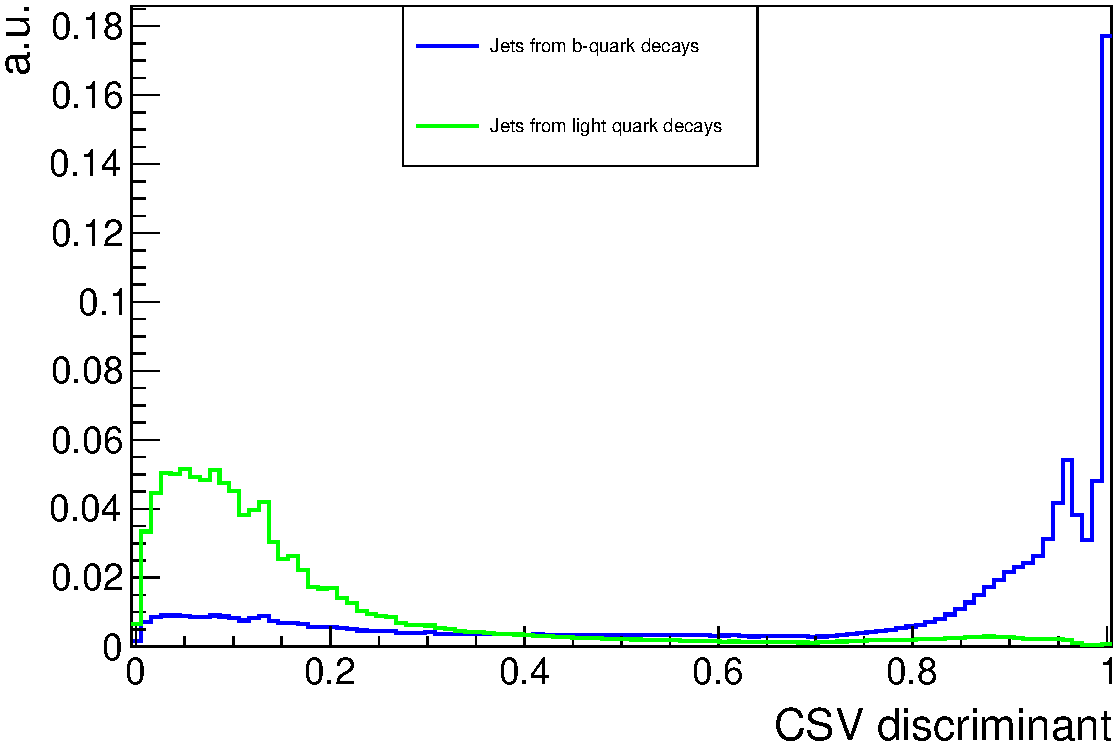
\includegraphics[width = 0.75 \textwidth]{Chapters/Chapter4_EvtSel/Figures/CSVDiscr_LightAndBJets.pdf}
 \caption{Combined Secondary Vertex b-tag discriminant for the different jet-flavours.} \label{fig::CSVDiscr}
 %*************************************
 % If possible, split this in a contribution of b, c, and light jets!
 %*************************************
\end{figure}

Since in this analysis priority is given to selecting event topologies which closely agree with the expected topology the double Tight CSV b-tagging requirement is expected to be the optimal choice.
This is indeed the case, the fraction of selecting the good jet combination increases from 0.409 up to 0.497 and finally reaches a value of 0.547 when tightening the CSV discriminant value from Loose to Tight. 
These fractions are determined from simulated semi-leptonic $\ttbar$ events for which information on the four generator-level partons corresponding to the four jets is available.
\\
It has also been investigated whether an improvement could be observed when the CSV discriminant of the light jet candidates is restricted, but since the effect was almost negligible it will not be considered further.
\\

After these double b-tagging requirement the background samples have been significantly reduced and the only remaining contribution comes from the single-top quark events, and then in particular the tW-channel.
The reason why this specific background process becomes relevant can be explained from a complex interplay between top-quark pair and single-top decays in the tW channel. This because the tW-channel single-top processes are well described at leading order but at next-to-leading order a set of Feynman diagrams is shared among both.
For this reason, a diagram-removal approach is applied in order to reduce the effect this overlap by not adding these type of diagrams in the tW-signal definition~\cite{DRST}.
%****************************
% --> Make sure it is interesting to keep this explanation!!
% --> Do not want tricky questions on this matter ...
% --> If kept, go through the cited paper!!
%****************************
\begin{figure}[h!t]
 \centering
 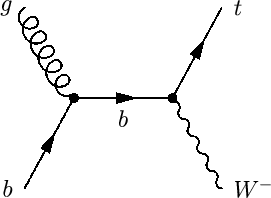
\includegraphics[width = 0.3 \textwidth]{Chapters/Chapter4_EvtSel/Figures/STtW_LO.png} \hspace{0.5cm}
 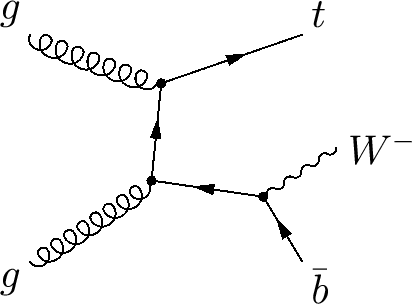
\includegraphics[width = 0.3 \textwidth]{Chapters/Chapter4_EvtSel/Figures/STtW_NLO.png}
 \caption{Leading-order (left) and next-to-leading (right) order Feynman diagram for tW production. The latter one corresponds to a leading-order diagram for top-quark pair production.} \label{fig::STtW}
\end{figure}

The application of this double Tight b-tagging algorithm is also the motivation why, besides the background samples discussed before, no other background contributions have been considered for this analysis as they will become completely redundant.

\subsection{Determining the optimal jet combination}
With the b-tag working point and the number of b-tags decided on, the topology reconstruction proceeds by assigning the selected jets to the final state particles expected in semi-muonic $\ttbar$ events.
This reconstruction procedure first identifies the two most energetic jets with sufficiently high CSV-discriminant value and labels all remaining jets as originating from light flavoured partons.
\\
For the two b-jet candidates should then be decided whether they originate from the top quark for which the W-boson decays into two jets, denoted as the hadronical decaying top quark, or from the top quark with the produced W-boson decaying into a muon and corresponding neutrino, the so-called leptonical decaying top quark.
This identification is important since it allows to reduce the number of permutations needed to be considered by the Matrix Element method.
From the collection of light jets only the two expected to originate from the hadronical decaying W-boson have to be identified, but not matched with a specific jet since the up- and down-type jet are difficult to be distinguished. %Hence the recovered event topology will have two possible permutations, which both have to be considered.
\\
\\
In this analysis, for which a high reconstruction efficiency is desired, it has been studied whether an improvement can be achieved when the two light-jet candidates are chosen from the three leading $\pT$ jets based on their kinematic resemblance in stead of using the more general approach of merely continuing with the two most energetic light jets.
This light-jet selection is performed simultaneously with the b-jet assignment and is based on a $\chi^{2}$-method using both the invariant mass of the lepton and the b-jet originating from the leptonical decaying top quark, denoted as $m_{lb}$, and the invariant mass of the full hadronic decaying top-quark system, $m_{qqb}$ or $m_{t}$.
\\
The expected values of these invariant masses have been determined by applying a Gaussian fit on the distribution obtained for all events passing the above-mentioned event selection requirements, resulting in $\hat{m}_{lb}$ =  107.79 $\pm$ 32.24 $\GeV$ and $\hat{m}_{qqb}$ = 175.03 $\pm$ 17.06 $\GeV$.
The benefit of using the $m_{lb}$ variable in stead of determining the invariant mass of the full leptonic decaying top-quark system is that the reconstruction of the neutrino can be avoided.
A small downside is the non-perfect Gaussian behaviour of this invariant mass distribution such that the fit had to be carefully applied onto a limited range of the distribution.
The obtained invariant mass distributions together with the Gaussian fit function are both given in Figure~\ref{fig::InvMasses}. %, from which the difference in shape is clearly visible.
\\
\begin{figure}[h!t]
 \centering
 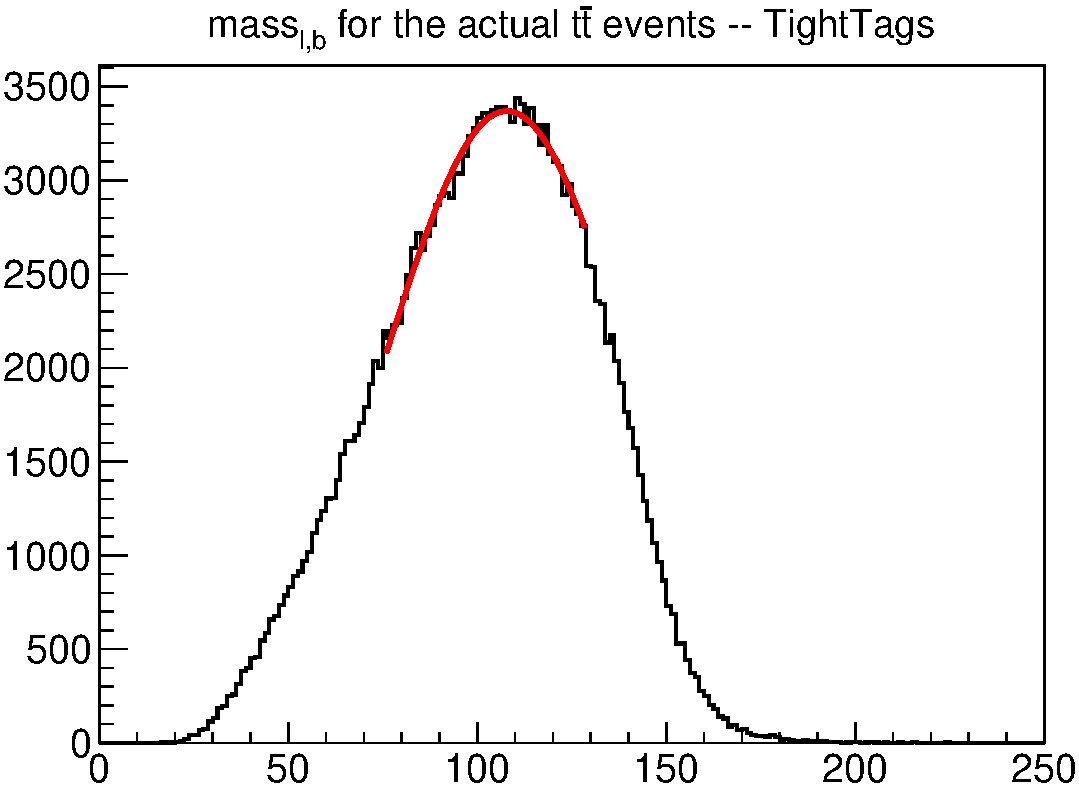
\includegraphics[width = 0.45\textwidth]{Chapters/Chapter4_EvtSel/Figures/MlbMassDistribution.pdf} %Mlb here
 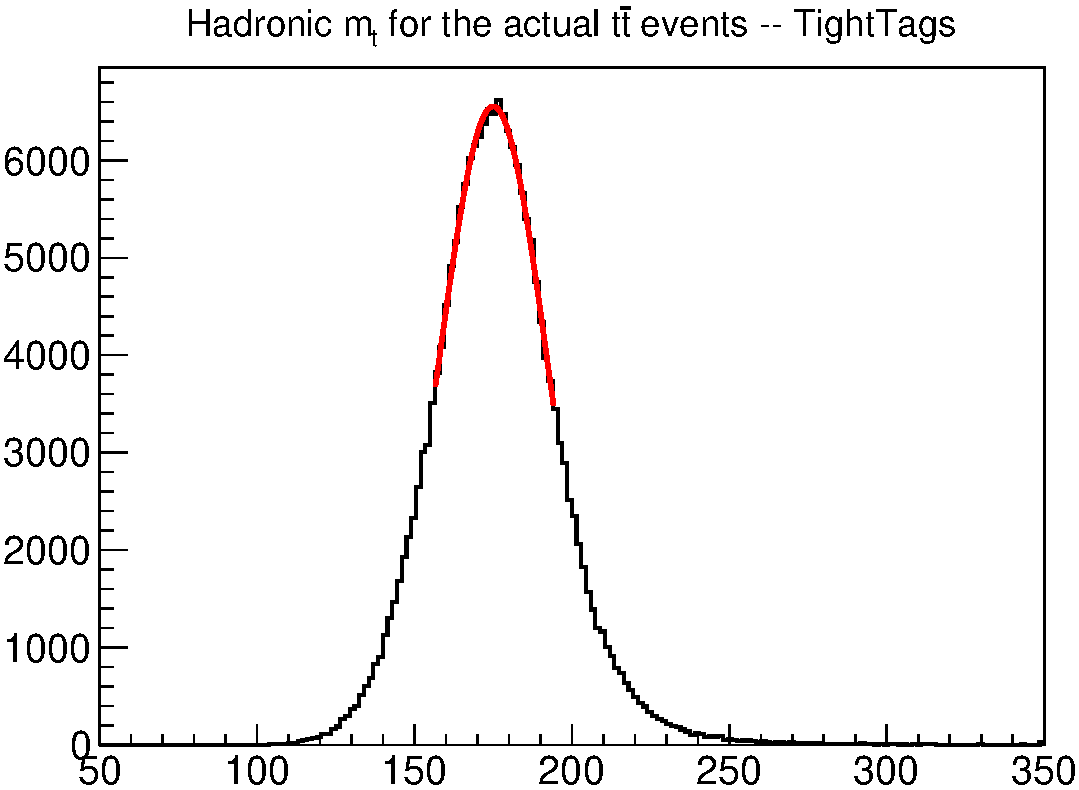
\includegraphics[width = 0.45\textwidth]{Chapters/Chapter4_EvtSel/Figures/HadrMTopMassDistr.pdf} %Mqqb here
 \caption{Distribution of the invariant masses, $m_{lb}$ on the left and $m_{qqb}$ on the right, together with the applied Gaussian fit function. The considered fit range corresponds to the $1\sigma$ interval.} \label{fig::InvMasses}
\end{figure}

In this analysis the most plausible jet assignment for the b-jets and the light jets is determined with the same $\chi^{2}$-based procedure for which the formula is given in Equation (\ref{eq::ChiSqMlbMqqb}).
For each event the $\chi^{2}_{i}$ value of the 6 possible jet combinations is calculated and the combination with lowest $\chi^2_{i}$ value is selected.
In case the considered event does not have a third jet present in the event, only the permutation between the hadronic and leptonic b-jet has to be taken into account.
\begin{equation} \label{eq::ChiSqMlbMqqb}
 \chi^{2}_{i} = \frac{(\hat{m}_{lb} - m_{lb,i})^{2}}{\sigma^{2}(\hat{m}_{lb})} + \frac{(\hat{m}_{qqb} - m_{qqb,i})^{2}}{\sigma^{2}(\hat{m}_{qqb})}
\end{equation}

Allowing the third light jet to be part of the chosen jet combination significantly improved the reconstruction efficiency and will therefore be applied in this analysis.
With these extra jet combinations to choose the most plausible one from, the possibility to select the correct two light jets increases from $63.13 \%$ to $76.21 \%$.
Due to this more correct determination of the light jet candidates the overall fraction of selecting good events, mentioned earlier to be 0.547, has improved to $0.666$.
This positive influence can also be seen when comparing the two distributions given in Figure~\ref{fig::ChiSq_4vs5Jets}. 
Here the left-handed figure contains the $\chi^{2}$ distribution for the chosen jet combination with and without the inclusion of this third jet, while the right-handed one shows the difference in shape of this $\chi^{2}$ distribution for the non-chosen jet combinations.
%improvement is also visible from the two $\chi^{2}$ distributions given in Figure~\ref{fig::ChiSq_4vs5Jets}, for which the left-handed one represents the $\chi^{2}$ distribution of the chosen jet combination with and without the inclusion of this third jet while the right-handed one describes the difference in shape of the wrong jet combinations $\chi^{2}$ for the same two options.
\begin{figure}[h!t]
 \centering
 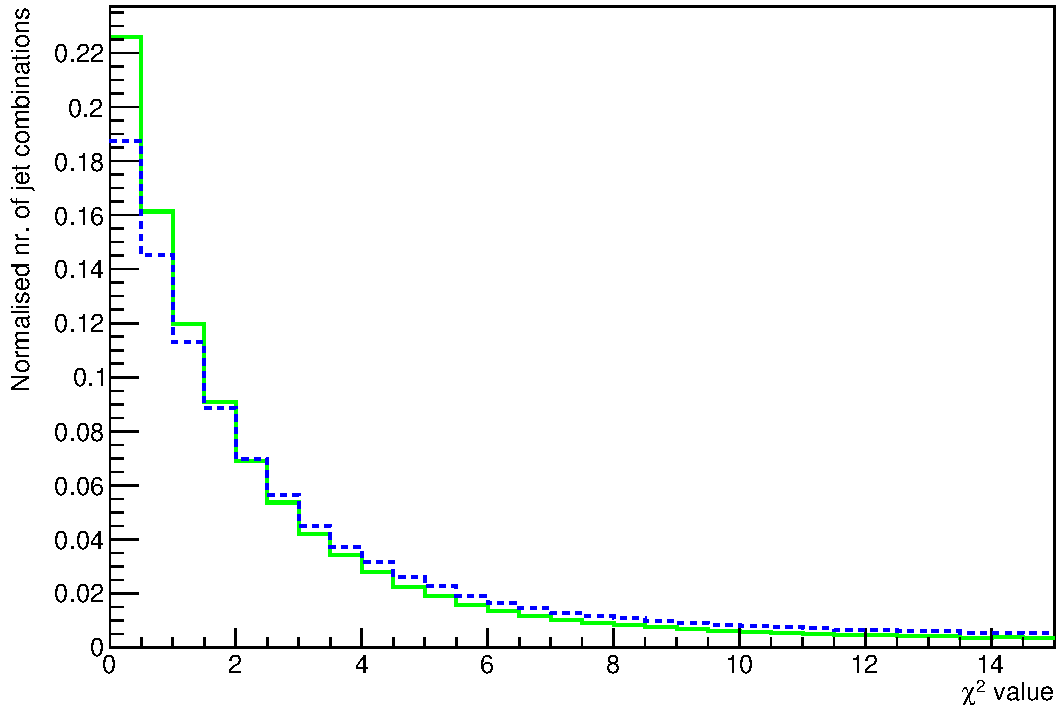
\includegraphics[width = 0.45 \textwidth]{Chapters/Chapter4_EvtSel/Figures/LowestChiSqComparison.pdf}
 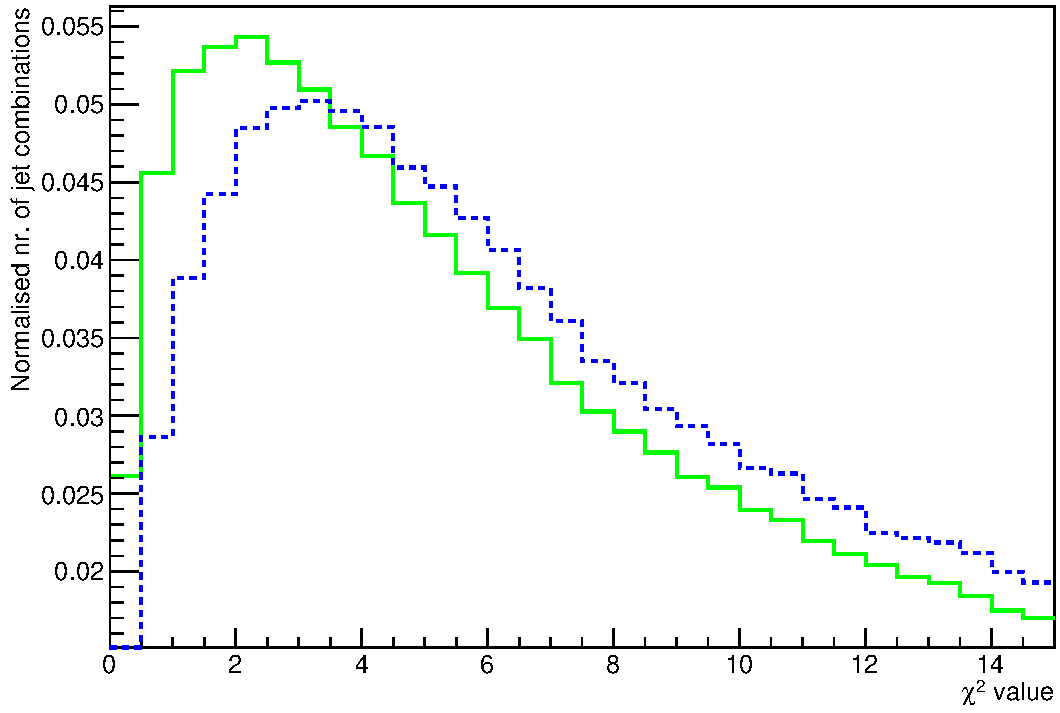
\includegraphics[width = 0.45 \textwidth]{Chapters/Chapter4_EvtSel/Figures/WrongChiSqComparison.pdf}    %Put here the same but for wrong chisqs (normalised to have comparable numbers!) 
 \caption{Comparison of the $\chi^{2}$ value of the chosen (left) and non-chosen (right) jet combinations. The solid green line represents the case where the third light-quark jet is allowed to be one of the candidate jets and the dashed black corresponds to the general approach of selecting the two leading light-quark jets.} \label{fig::ChiSq_4vs5Jets}
 %\caption{... can maybe also plot the normalised shape of the wrong combinations ... -- need solid and dashed line!!} 
\end{figure}
%******************
% Question: necessary to add pileup to numbers?
%******************

\subsection{Improving the topology reconstruction}\label{subsec::MassCuts}
Even though the application of a b-jet identification algorithm will significantly reduce the different background contributions, some improvement can still be obtained by excluding events using specific kinematic criteria, as will be demonstrated here. This will in addition ameliorate the reconstruction efficiency, two conditions which are both beneficial for this analysis.
This follows from the fact that the Matrix Element method treats all events as it were semi-leptonical top-quark pair decays such that a definite gain can be achieved when the possibility to choose the correct event topology is enhanced.
\\
Therefore two additional event selection criteria have been considered, both relying on the invariant mass distributions. %(of the hadronical and leptonical decaying top-quark system.)
At first the hadronical decaying top-quark system is restricted by requiring the reconstructed invariant masses, $m_t$ and $m_W$, to lie within a predefined number of standard deviations from the expectation. Secondly a limitation of the $\chi^{2}$ variable, using information from both top quarks as shown in Equation (\ref{eq::ChiSqMlbMqqb}), has been studied.
As these two procedures use an overlapping variable to reject undesired events, the invariant mass $M_{lb}$, a correlation between the two is expected.
This correlation, $\chi^{2}$ and $m_{t}$ on the one hand and $\chi^{2}$ and $m_{W}$ on the other hand, can be visualised in Figure~\ref{fig::2Dexclusion}.

\begin{figure}[h!t]
 \centering
 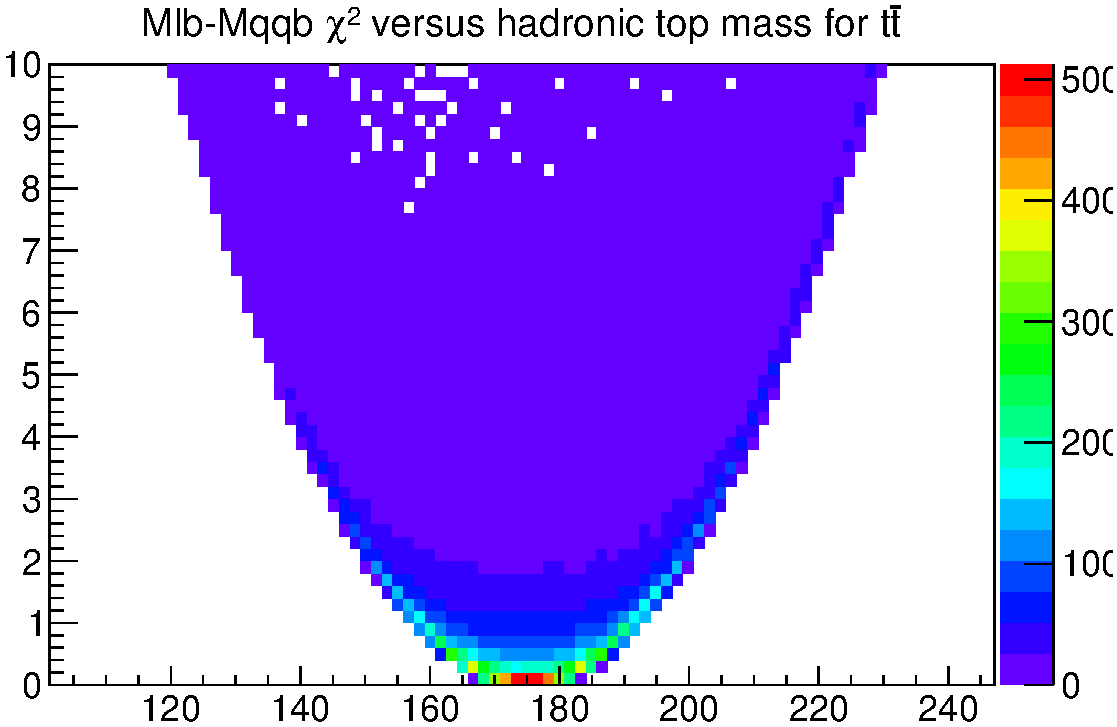
\includegraphics[width = 0.45 \textwidth]{Chapters/Chapter4_EvtSel/Figures/MqqbVSChiSq.pdf} %ChiSq vs numbers of sigma deviation from top-mass here (abs value)
 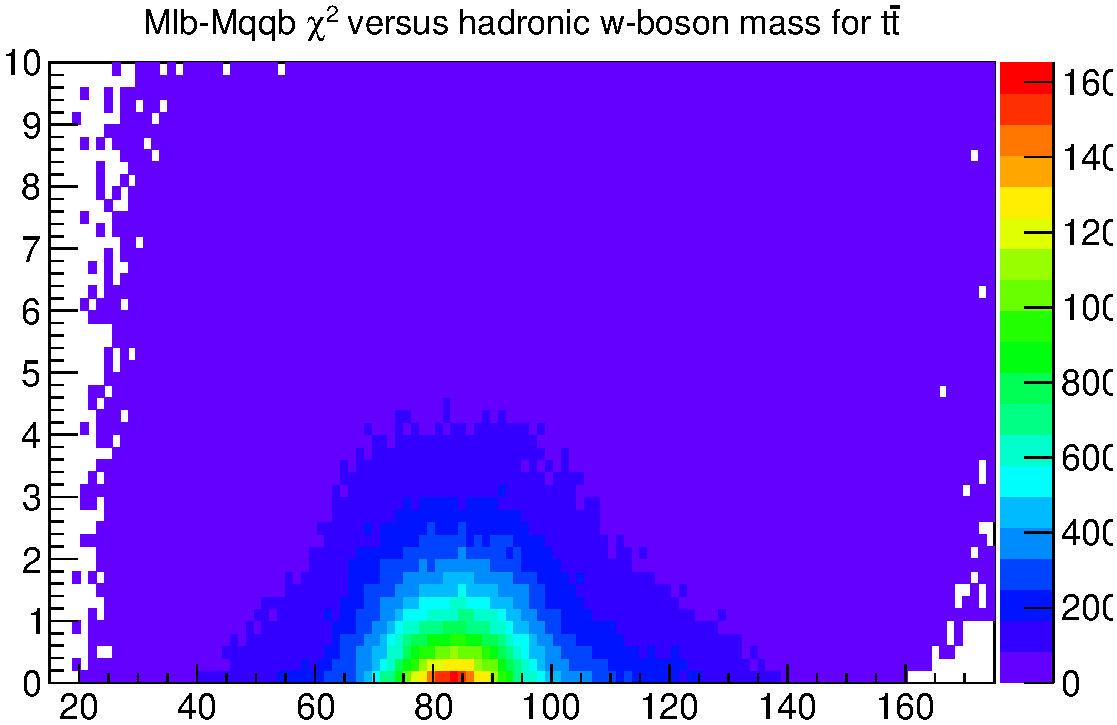
\includegraphics[width = 0.45 \textwidth]{Chapters/Chapter4_EvtSel/Figures/MlbVSChiSq.pdf} %ChiSq vs numbers of sigma deviation from W-mass here (abs value)
 \caption{Correlation between the $\chi^{2}$-value of the chosen jet combination and the invariant mass of the jets forming the hadronic top-quark (left) and W-boson topology (right).} \label{fig::2Dexclusion}
\end{figure}

Restricting the mass values of both the hadronical decaying top quark and the W-boson is a rather effective manner of ensuring the reconstructed top-quark topology actually corresponds to a $\ttbar$ decay.
%In order to apply both mass constraints simultaneously, it has been decided to use the measured mass values together with a specific number of standard deviations to create an allowed mass range.
The expected W-boson mass has been determined by fitting the obtained invariant mass distribution after all event selection criteria have been applied with a Gaussian function, as was the case for the top-quark mass in the $\chi^{2}$-based method ($\hat{m}_{t}$ = $175.03$ $\pm$ $17.06$ $\GeV$). For the W-boson mass this resulted in a value of $\hat{m}_{W}$ $=$ $83.62$ $\pm$ $17.06$ $\GeV$, retrieved from the distribution given in Figure~\ref{fig::InvWMass}.
\\
%It has been determined that 
The optimal cut-value, which sufficiently improves the reconstruction efficiency without drastically reducing the event count, has been identified as the $2\sigma$ interval. For this mass range the number of selected semi-leptontic $\ttbar$ events fulfilling the double b-tag requirement is halved while the reconstruction fraction has increased to 0.791.
%corresponds to an allowed number of standard deviations of 2. 
\begin{figure}[h!t]
 \centering
 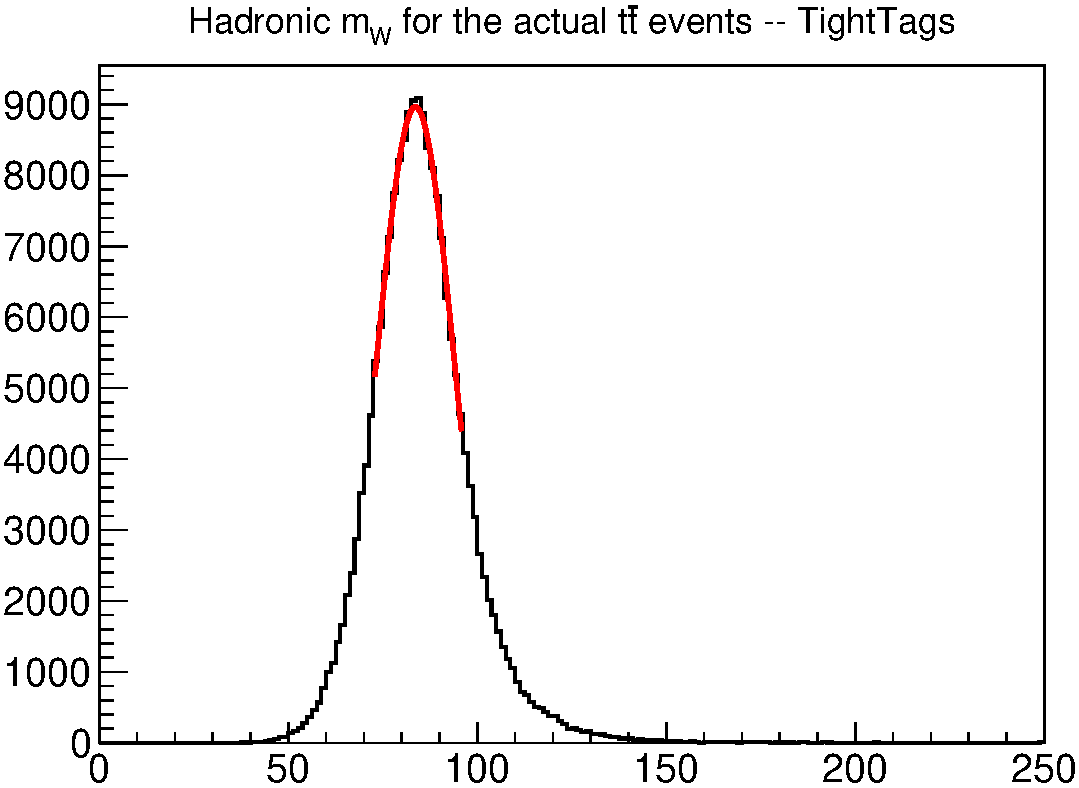
\includegraphics[width = 0.7 \textwidth]{Chapters/Chapter4_EvtSel/Figures/HadrMWMassDistr.pdf}  %Put here the MW mass distribution (but do not make it too large ...)
 \caption{Distribution of the invariant mass of the hadronic W-boson, $m_{W}$, together with the applied Gaussian fit function. Also here, the considered fit range corresponds to the $1\sigma$ interval.} \label{fig::InvWMass}
\end{figure}

The second considered requirement, limiting the $\chi^{2}$ variable of the chosen jet combination, aims to exclude the events unlikely to be properly reconstructed.
For the events residing in the tail of this $\chi^{2}$ distribution the possibility to correctly assign all four jets to the considered event topology is as low as 20 $\%$.
In order to ensure the $\chi^{2}$ restriction results in a cleaner event sample without rejecting the majority of the events, as was the case for the invariant mass constraint, the cut-value to be fulfilled for the chosen jet combination is $\chi^{2}$ $<$ $10$.
Without the mass restrictions being applied, this requirement slightly enhances the reconstruction to 0.699 while reducing the event count for the considered simulated semi-leptonic $\ttbar$ sample with 23 $\%$.
\\

The overall effect of these two additional event selection criteria will have less of on impact on the final result than the b-jet identification algorithm, but is nonetheless an efficient way to reduce the contribution of poorly reconstructed events.
When demanding both the invariant mass and the $\chi^{2}$ restriction to be fulfilled, the possibility to correctly reconstruct the entire top-quark pair event topology reaches a value of $79.33\%$.
The small improvement compared to the individual results, mainly dominated by the mass requirement, can be understood from the large correlation between both methods.
%The high correlation between both methods explains why the combined application does not strongly enhance the reconstruction efficiency obtained individually.
%Since both methods are highly correlated it is not expected that their combined application will strongly enhance the reconstruction efficiencies already achieved individually. However, a very small %improvement is still obtained 

\section{Influence of full event selection} %Kinematics of remaining events/Finalized event selection}\label{sec::DataMC} 
The full event selection consists of the triggering and cleaning conditions discussed in Section~\ref{sec::MainSelec} combined with the analysis-specific supplementary fine-tunings introduced in Section~\ref{sec::SpecificSelec}.
The additional event selection criteria applied here have all been developed with the intention to reduce the contribution from the different background processes while remaining with a selected sample dominated by well reconstructed events.
This goal is clearly achieved under the influence of the considered selection requirements
%, 2 jets fullfilling the Tight Combined Secondary Vertex b-tagging requirement; $\chi^{2}$-value of the chosen jet-combination choice smaller than 10; and both the reconstructed top-quark and W-boson mass located within the $2\sigma$ interval around its expectation value, 
since for 79.33$\%$ of the semi-leptonic $\ttbar$ events the correct jet assignment is chosen.
\\

The selected sample of both simulated and data events are determined using the same event selection criteria and, before the actual analysis can be carried out, a detailed comparison between the two is performed to ensure the data is well described by the considered simulated samples.
%With the full event selection finalized, a comparison between data and simulation is a practical tool to ensure the considered background processes are sufficient to describe the studied interaction.
In order for this comparison to be correct, the different calibrations accounting for the different response of data and simulated events in specific conditions have to be applied.
%However, before such an agreement can be achieved, the different calibrations need to be applied to simulation to account for the minor discrepancies between data and simulated events.
\\
\\
%At first the simulation has to be reweighted in order to correctly describe the number of pileup interactions.
As has been explained in Section~\ref{sec::DetectorSim}, the simulation samples are generated using a distribution for the number of pileup interactions meant to correspond with the expected conditions for the considered data-taking period. However, these conditions might vary slightly and thus need to be corrected for once the exact pileup information in data is known.
Therefore the number of pileup interactions in simulation is reweighted to the distribution observed in data using a luminosity-based pileup estimate.
This method determines the total number of interactions in each bunch crossing from the measured instantaneous luminosity for the corresponding bunch crossing and the total inelastic proton-proton collision cross-section.
%**********************************
% Info found on: https://twiki.cern.ch/twiki/bin/view/CMS/PileupJSONFileforData
%  --> Any reference somewhere??
%**********************************
\\
\\
The second calibration that needs to be applied corrects for the slightly different efficiency of the b-jet identification algorithm in data and simulation~\cite{BTagSF}.
This aspect has been studied in great detail and has resulted in the development of b-tag efficiency scale-factors, analytic functions depending on the transverse momentum of the jets, to account for these discrepancies by correcting the measured jet-dependent efficiencies in simulation.
%**********************
%Important to note: No eta-dependency for Tight CSV!
%**********************
%\textit{This results in an overall event probability as expected in data, which can then be compared to the corresponding event efficiency in simulation.}
%\textit{The in this way determined event-weight is thus analysis-specific since it will only use events passing the selection requirements.}
\\
The determination of the b-tag event-weight starts by computing the efficiency $\varepsilon_{f}$ for a jet of flavour $f$ to be identified as a b-jet using simulated semi-leptonic $\ttbar$ events.
From these efficiencies an overall event probability $P_{sim}$ can be calculated by multiplying the efficiencies of all jets residing in the event\footnote{It is important to note that in Equation (\ref{eq::PSim}) the labels \textit{tagged} and \textit{non-tagged} refer to whether the considered jet fulfilled the applied b-tag requirement and not whether it has been labelled as one of the two b-jet or light jet candidates in the event selection.}, as shown in Equation (\ref{eq::PSim}).
The corresponding event probability as expected in data, $P_{data}$ in Equation(\ref{eq::PData}), is determined in the same way, but every jet-efficiency is corrected using the aforementioned scale-factor $SF$.
%****************************************
% Remark: If b-tag is leading systematic the SF distributions can maybe be added as a plot!!
%****************************************
\begin{eqnarray} 
 P_{sim} & = & \prod_{i = tagged} \varepsilon_{i} \prod_{j = non-tagged} (1-\varepsilon_{j})  \label{eq::PSim} \\
 P_{data} & = & \prod_{i = tagged} SF_{i} ~ \varepsilon_{i} \prod_{j = non-tagged} (1- SF_{j} ~ \varepsilon_{j}) \label{eq::PData}
\end{eqnarray}
From these two probabilities the overall event-weight can be determined in a straightforward manner by comparing the probability for data with the one in simulation:
\begin{equation}
 \textrm{event-weight } w = \dfrac{P_{data}}{P_{sim}}
\end{equation}

Once all necessary calibrations have been included the actual comparison between data and simulation can be performed at a luminosity of 19.6 $\pm$ xx $\fbinv$, which is the amount of data collected by the considered isolated-muon triggers during the 2012 data-taking period.
%The trigger paths applied in this analysis, based on a single isolated muon, collected a total of 19.6 $\pm$ xx $\fbinv$ during the 2012 data-taking period.
The final number of events obtained after demanding both the data and the simulated samples pass through the complete event-selection chain are given in Table~\ref{table::DataMCComp}.
As expected, the background contribution is almost negligible due to the stringent event-selection criteria.
%Once all the necessary calibration factors have been applied the actual comparison between data and simulated events can be performed.
%To start Table contains the obtained event numbers for data and all of the considered simulation samples after \textit{sending through} the full event selection.
\begin{table}[h!t]
 \caption{Event count obtained after applying the full event-selection chain for data together with the expected values and corresponding statistical uncertainties in simulation.} \label{table::DataMCComp}
 %The given uncertainties are purely statistical and demonstrate the limited size of the different samples} \label{table::DataMCComp}
 \centering
 \begin{tabular}{c|c}
  \hline
  Sample 			& Number of events 	\\
  \hline
  \hline
  Semi-leptonic $\ttbar$ 	& 16173 $\pm$ 41 	\\
  W+jets 			& 66 $\pm$ 7		\\
  Z+jets 			& 17 $\pm$ 4		\\       %Also photon here????????
  Single top 			& 359 $\pm$ 24		\\
  \hline
  Total				& 16 615 $\pm$ 76	\\
  \hline
  \hline
  Observed			& 16943			\\
  \hline
 \end{tabular}
\end{table}

The considered calibrations both influence the individual event kinematics and therefore modify the shape of the kinematic distributions.
The overall event count obtained in simulation, however, is not affected by the pileup reweighting since this correction factor averages out to unity.
The importance of this correction can be visualised in Figure~\ref{fig::PUInfl}, which contains the primary vertex multiplicity with and without this specific reweighting applied.
Comparing the two distributions clearly illustrates a better shape description, and thus significantly improved agreement between data and simulation, when taking into account the calibration factor.
\\
The b-tag event-weight, on the other hand, has an average value of only 0.87 $\pm$  (\textbf{Get the uncertainty from up/down}), mainly due to the stringent requirement of demanding two jets to fulfil the Tight working-point requirement of the CSV algorithm.
Hence the event count in simulation has largely been overestimated and is therefore scaled down in order to correctly take into account the difference in b-jet identification efficiency.
%The uncertainty on this latter scale-factor also largely covers the small statistical disagreement which exists between data and simulation, as can be seen from Table~\ref{table::DataMCCompBTag}.
%\\
%\begin{table}[h!t]
% \caption{TITLE} \label{table::DataMCCompBTag}
% \centering
% \begin{tabular}{c|c|c}
%  \hline
%  \multirow{2}{*}{Sample} 	& \multicolumn{2}{c}{Number of events} 	\\
%				& Statistical uncertainty & b-tag uncertainty \\
%  \hline
%  \hline
%  $\ttbar$ 			& separate or combined?	& useful? \\
%  W+jets 			& 			& \\
%  Z+jets (why $\gamma$?)	& 			& \\
%  Single top 			& 			& \\
%  \hline
%  Total				& 			& \\
%  \hline
%  \hline
%  Observed			&			& \\
%  \hline
% \end{tabular}
%\end{table}
%
%The relative contribution of the three calibrations can be visualized \textbf{from/in} Figures~\ref{fig::PUInfl} - \ref{fig::BTagInfl}, where each time one of the more relevant distributions is given before and after the specific scale-factor is applied. 
%
%The first Figure (\textit{include this way?}) contains the primary vertex multiplicity, the variable altered by the pileup reweighting procedure, and clearly illustrates the importance of this calibration factor since the shape is much better described after the reweighting resulting in a significantly improved Data/MC agreement.
%Secondly the influence of the lepton scale-factor is described using the distribution of the transverse momentum of the selected muon. 

\begin{figure}[h!t]
 \centering
 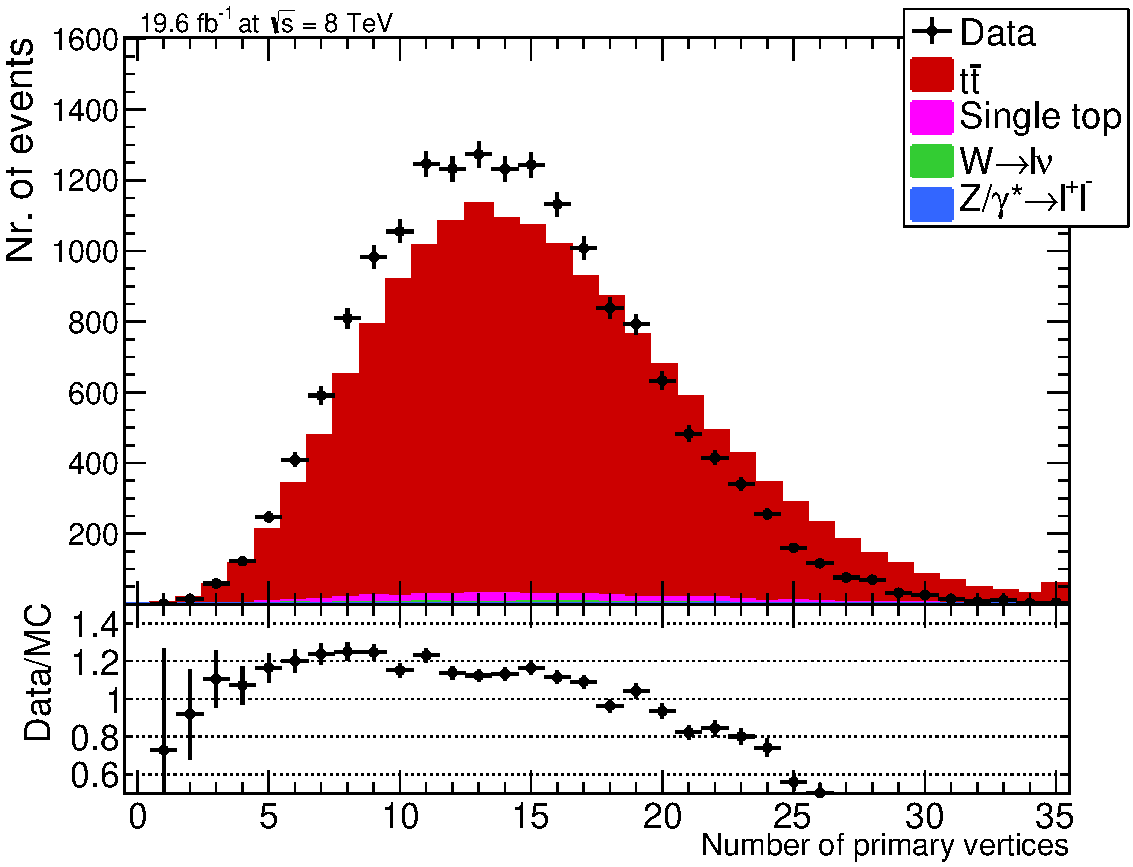
\includegraphics[width = 0.45 \textwidth]{Chapters/Chapter4_EvtSel/Figures/nPV_AllCuts_noPU_mu_Stack.pdf}
 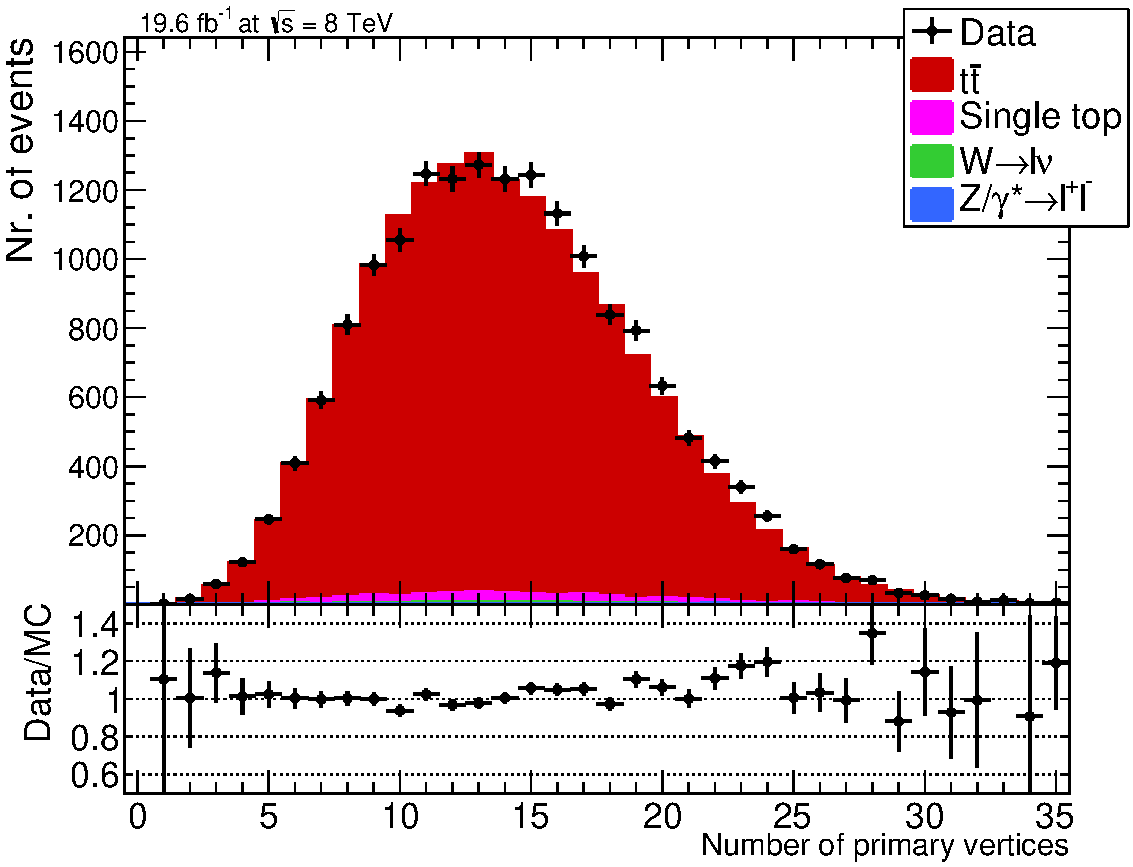
\includegraphics[width = 0.45 \textwidth]{Chapters/Chapter4_EvtSel/Figures/nPV_AllCuts_mu_Stack.pdf}
 \caption{Distribution of the number of primary vertices before and after the pileup reweighting is applied.} \label{fig::PUInfl}
 % Still need to change the x-axis to go from -0.5 to 35.5!
\end{figure}

The right-handed distribution in Figure~\ref{fig::PUInfl} nicely confirms the good agreement obtained between data and simulation after applying the full event selection chain and introducing the necessary calibration factors. This is also perfectly visible in other kinematic variables, and some of the more relevant ones for the discussed analysis will now be given.
\\
The different distribution chosen to be displayed are the transverse momentum $\pT$ and pseudo-rapidity $\eta$ of the four reconstructed jets using the techniques discussed in Section~\ref{sec::SpecificSelec} and the selected muon. These two kinematic variables serve as input for the Matrix Element Method for which the details will be discussed in Chapter~\ref{ch::MW}.
%To finalize this chapter some of the more important variables for this analysis will be given.
\begin{figure}[h!t]
 \centering
 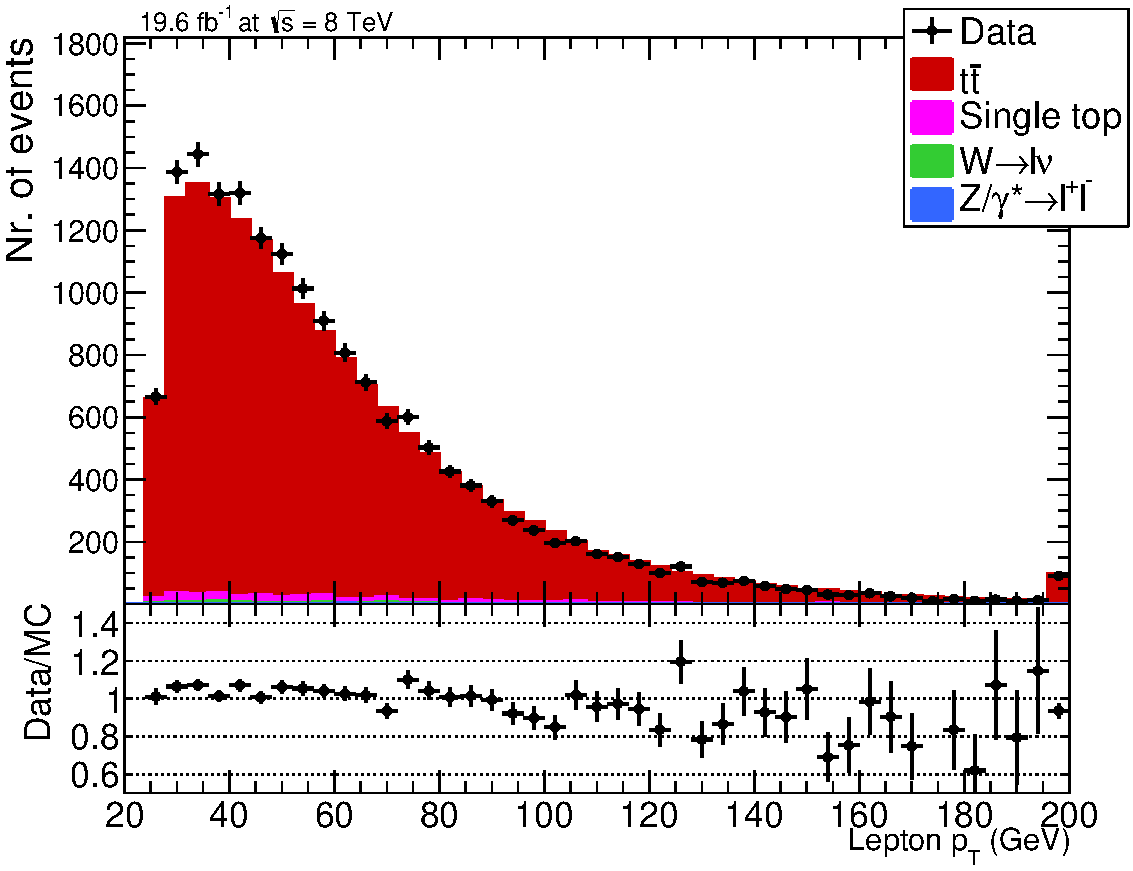
\includegraphics[width = 0.45 \textwidth]{Chapters/Chapter4_EvtSel/Figures/LeptonPt_AllCuts_mu_Stack.pdf}
 %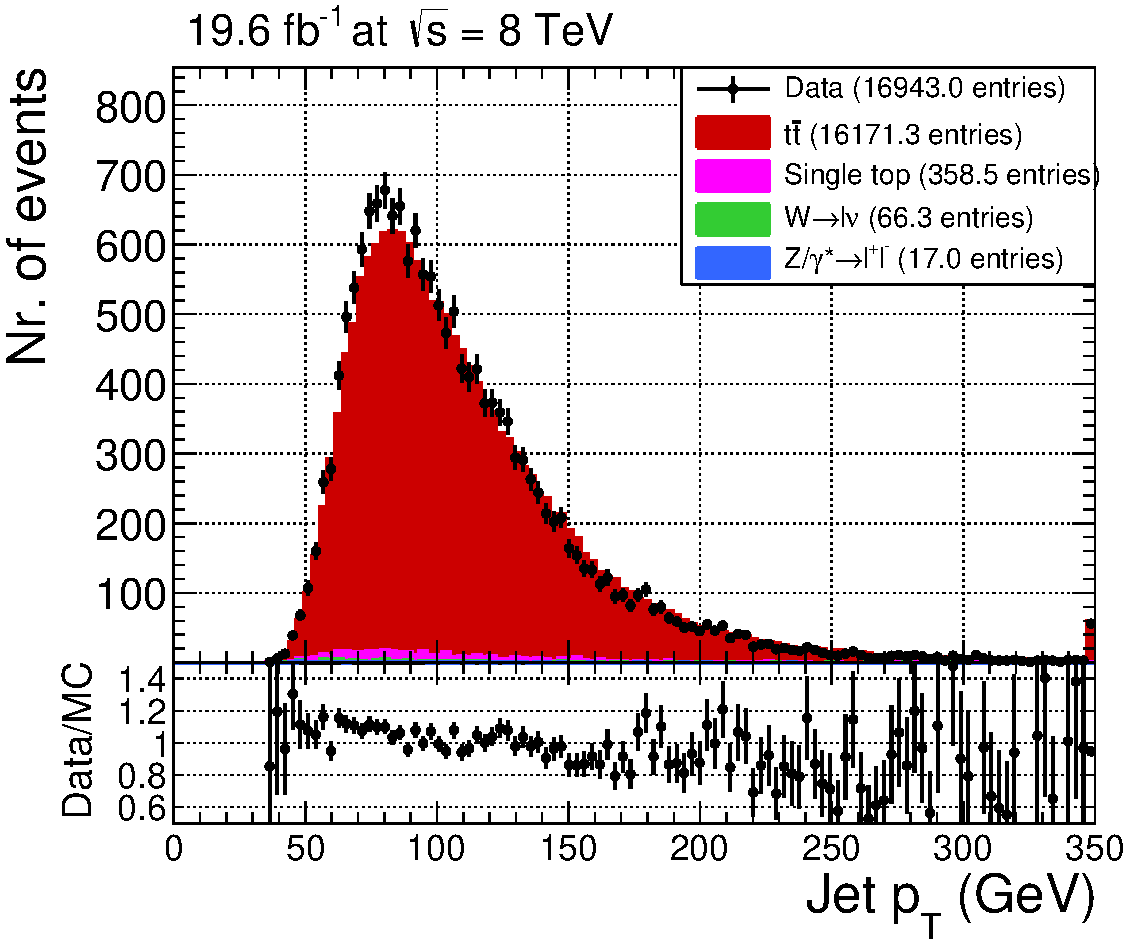
\includegraphics[width = 0.45 \textwidth]{Chapters/Chapter4_EvtSel/Figures/JetPt_LeadingJet_AllCuts_mu_Stack.pdf}
 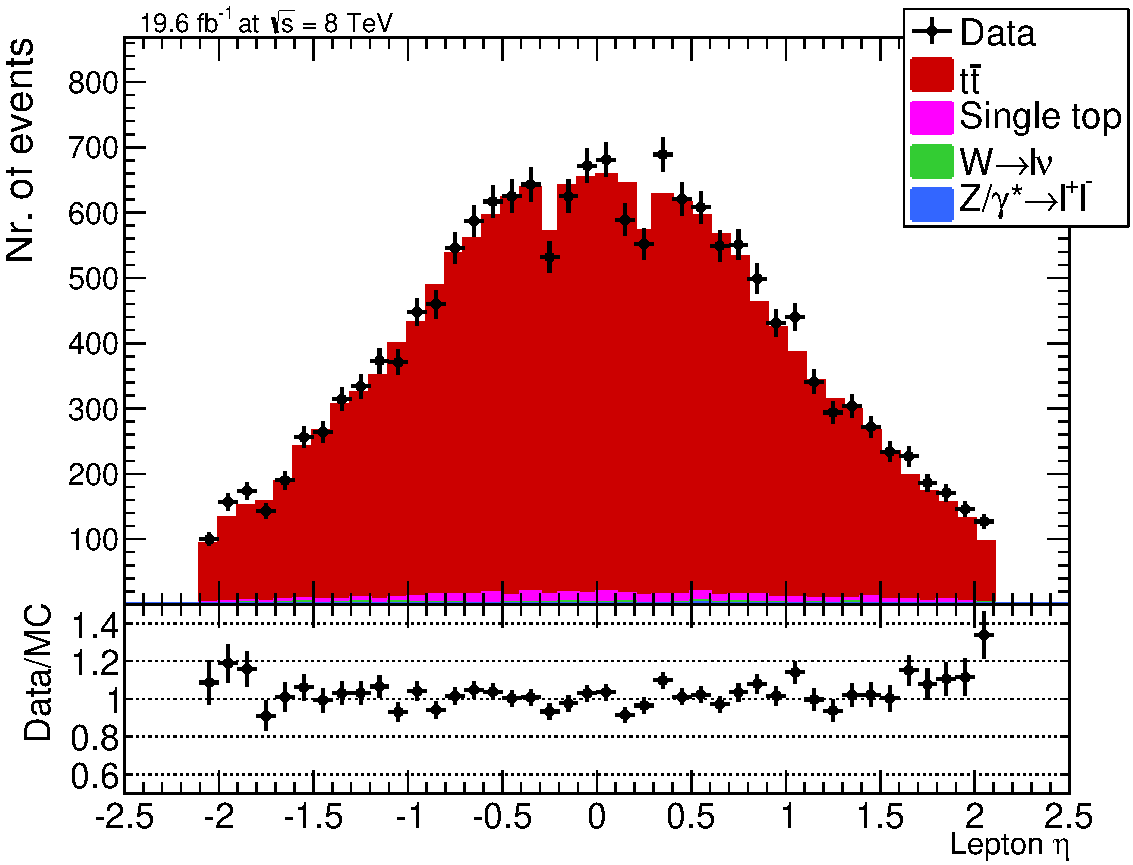
\includegraphics[width = 0.45 \textwidth]{Chapters/Chapter4_EvtSel/Figures/LeptonEta_AllCuts_mu_Stack.pdf}
 %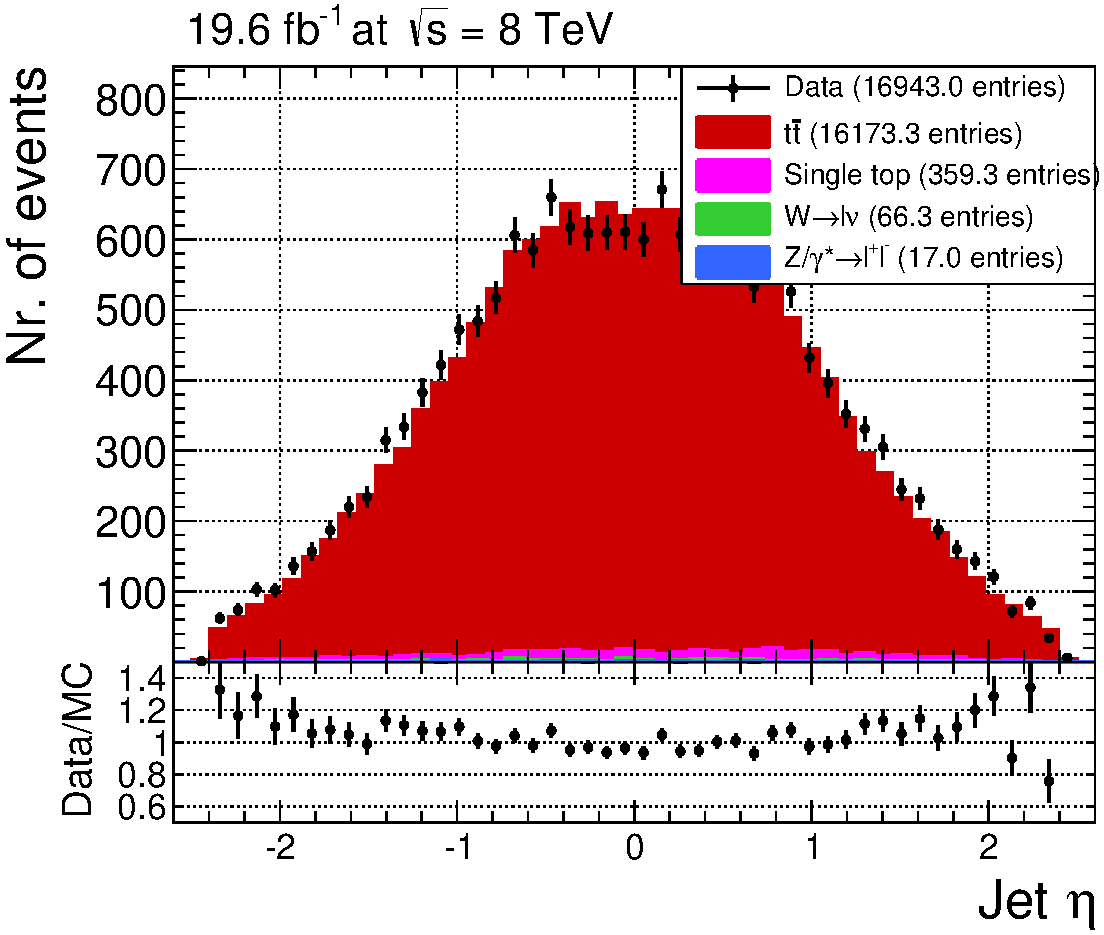
\includegraphics[width = 0.45 \textwidth]{Chapters/Chapter4_EvtSel/Figures/JetEta_LeadingJet_AllCuts_mu_Stack.pdf}
 \caption{Comparison between data and simulation for the lepton transverse momentum (left) and pseudo-rapidity (right).} \label{fig::MSPlots}
\end{figure}

\begin{figure}[h!t]
 \centering
 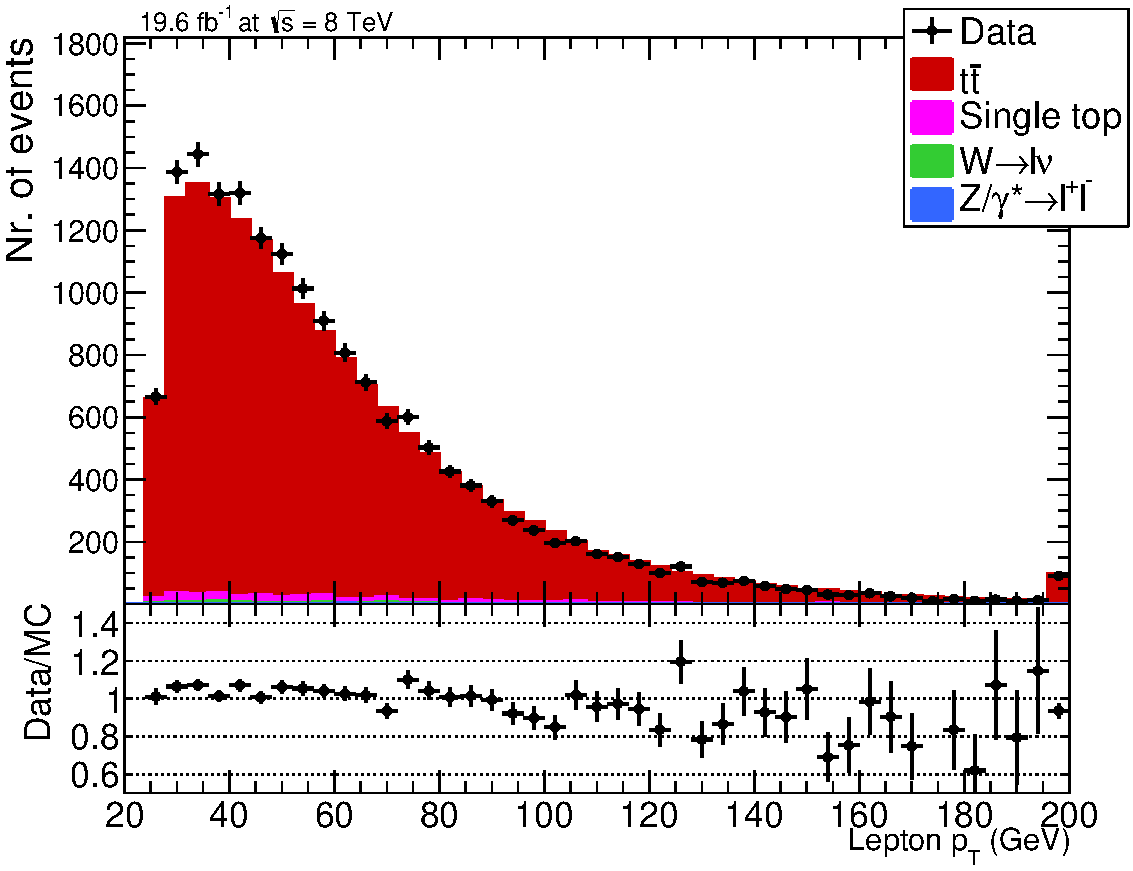
\includegraphics[width = 0.45 \textwidth]{Chapters/Chapter4_EvtSel/Figures/LeptonPt_AllCuts_mu_Stack.pdf}
 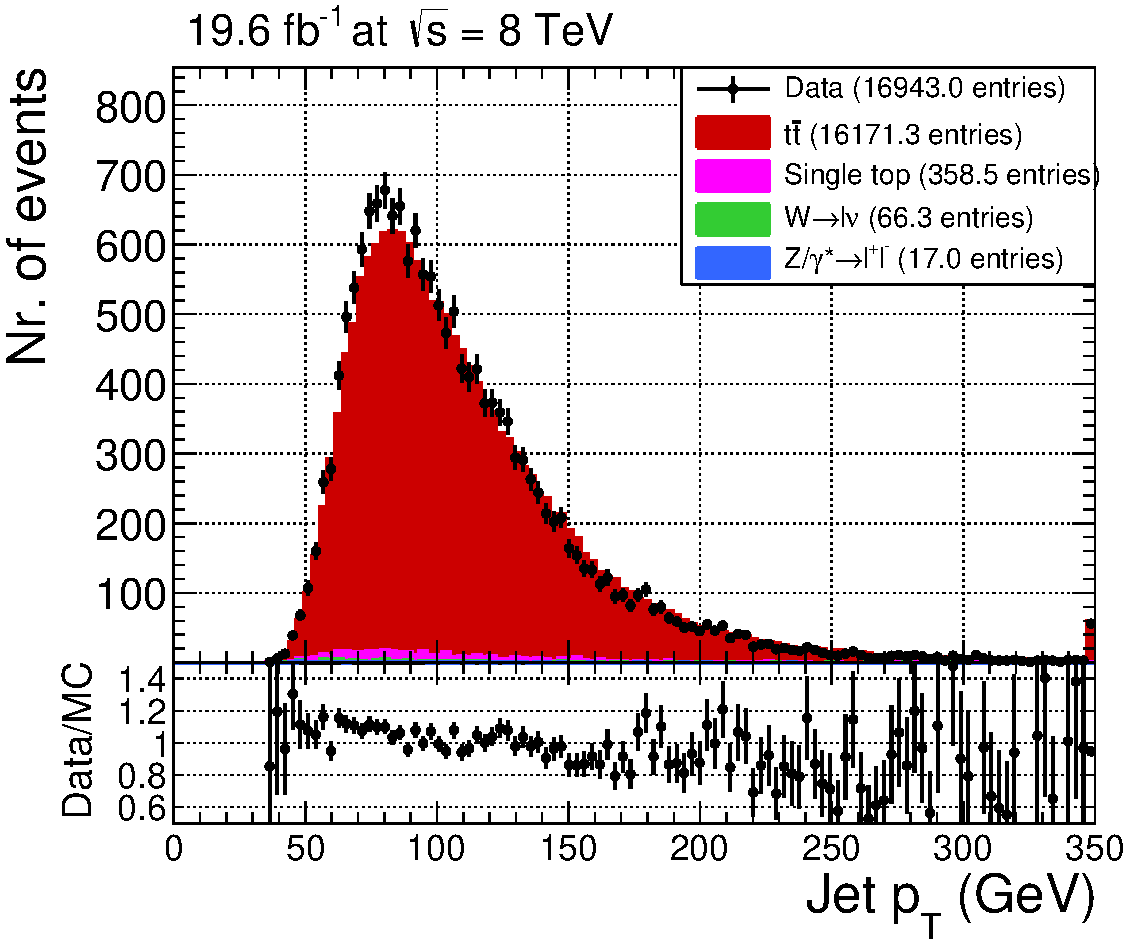
\includegraphics[width = 0.45 \textwidth]{Chapters/Chapter4_EvtSel/Figures/JetPt_LeadingJet_AllCuts_mu_Stack.pdf}
 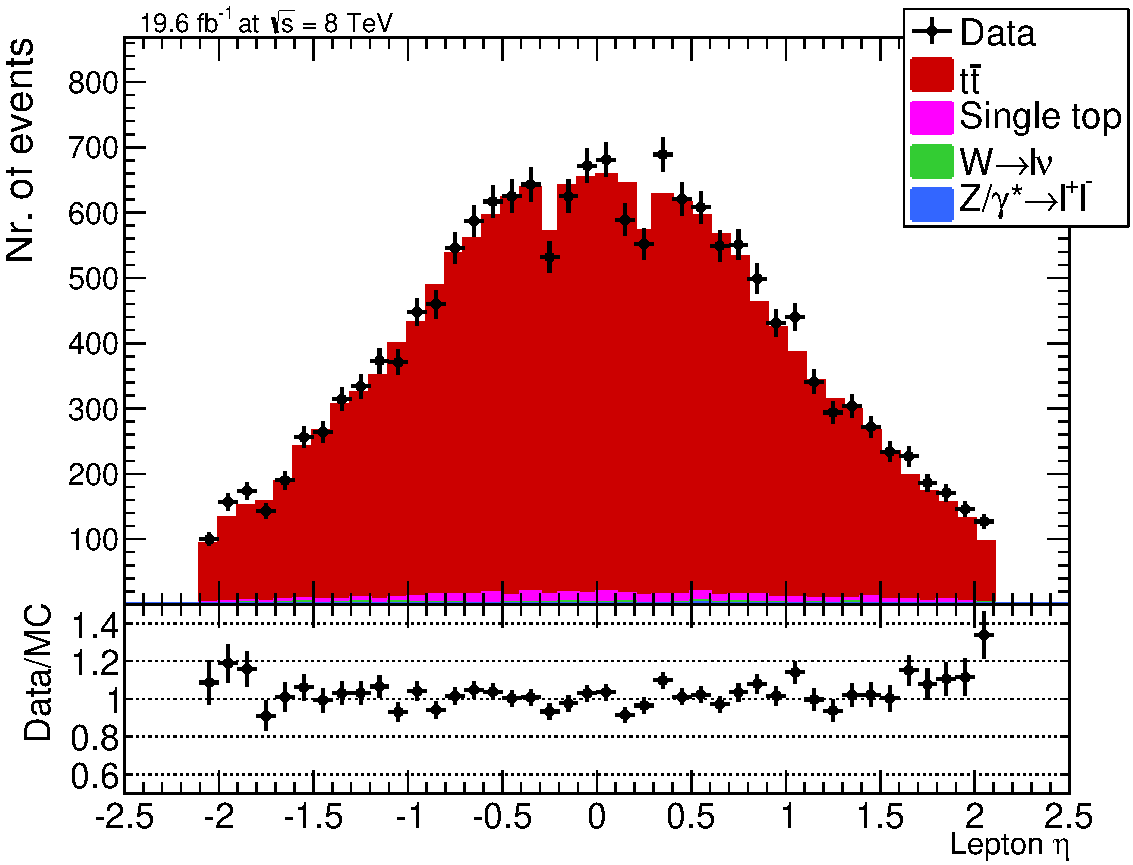
\includegraphics[width = 0.45 \textwidth]{Chapters/Chapter4_EvtSel/Figures/LeptonEta_AllCuts_mu_Stack.pdf}
 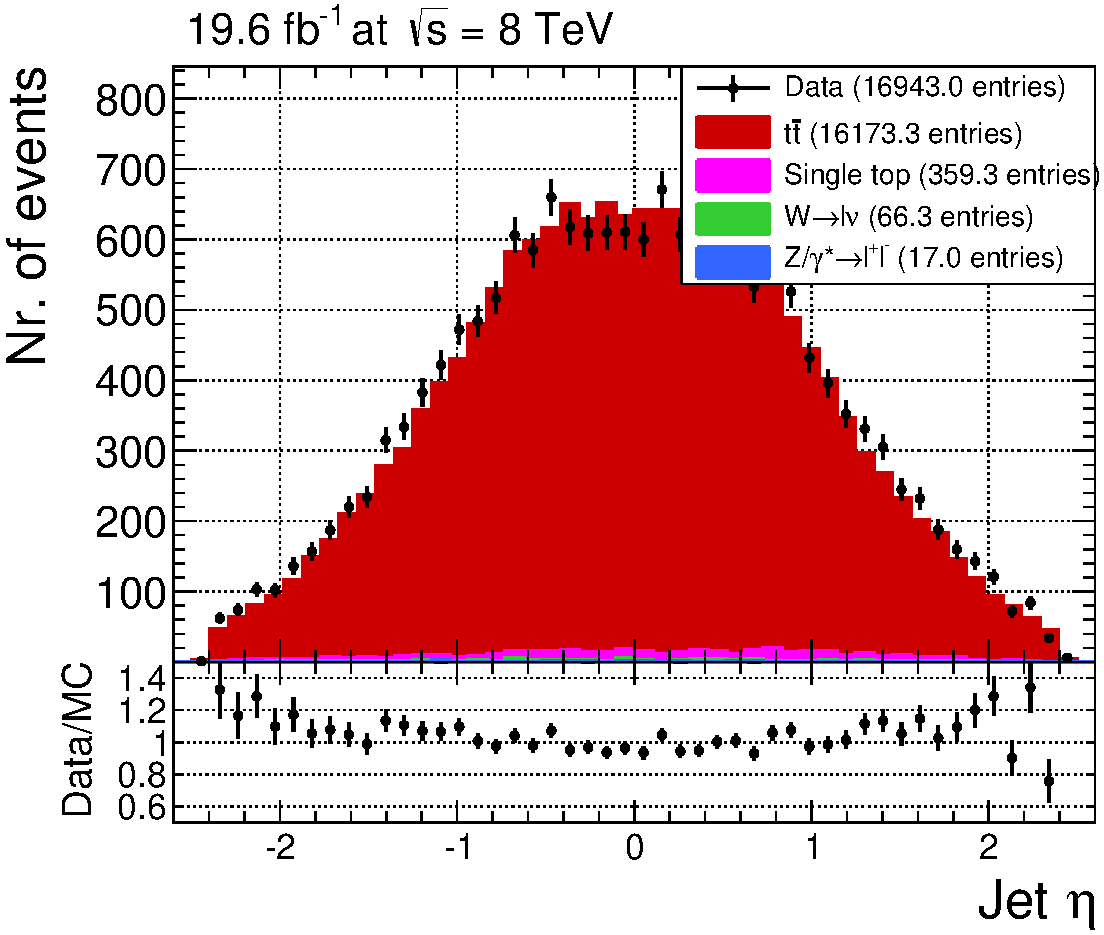
\includegraphics[width = 0.45 \textwidth]{Chapters/Chapter4_EvtSel/Figures/JetEta_LeadingJet_AllCuts_mu_Stack.pdf}
 \caption{Comparison between data and simulation for the lepton transverse momentum (left) and pseudo-rapidity (right) for the two reconstructed b-jets. The properties of the b-jet originating from the hadronic decaying top-quark are described in the upper distributions and the leptonic b-jet in the lower ones.} \label{fig::MSPlots}
\end{figure}

\begin{figure}[h!t]
 \centering
 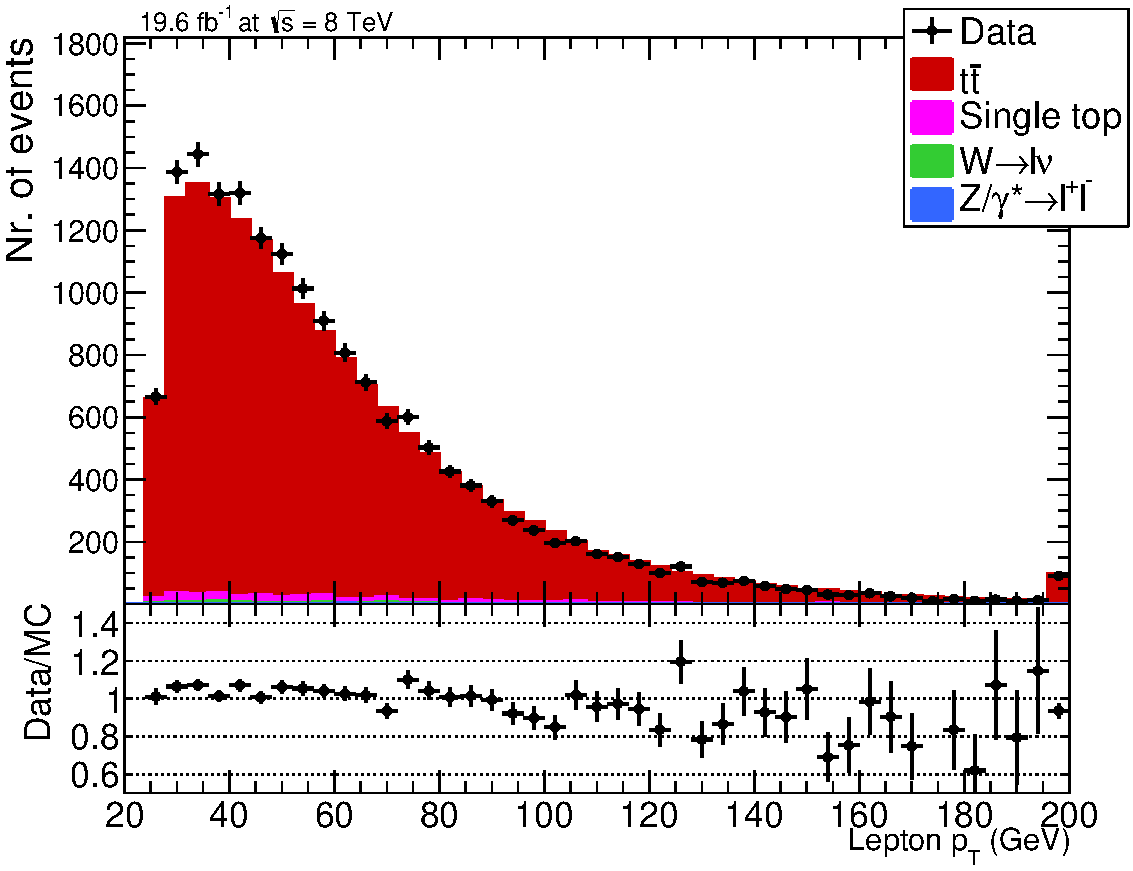
\includegraphics[width = 0.45 \textwidth]{Chapters/Chapter4_EvtSel/Figures/LeptonPt_AllCuts_mu_Stack.pdf}
 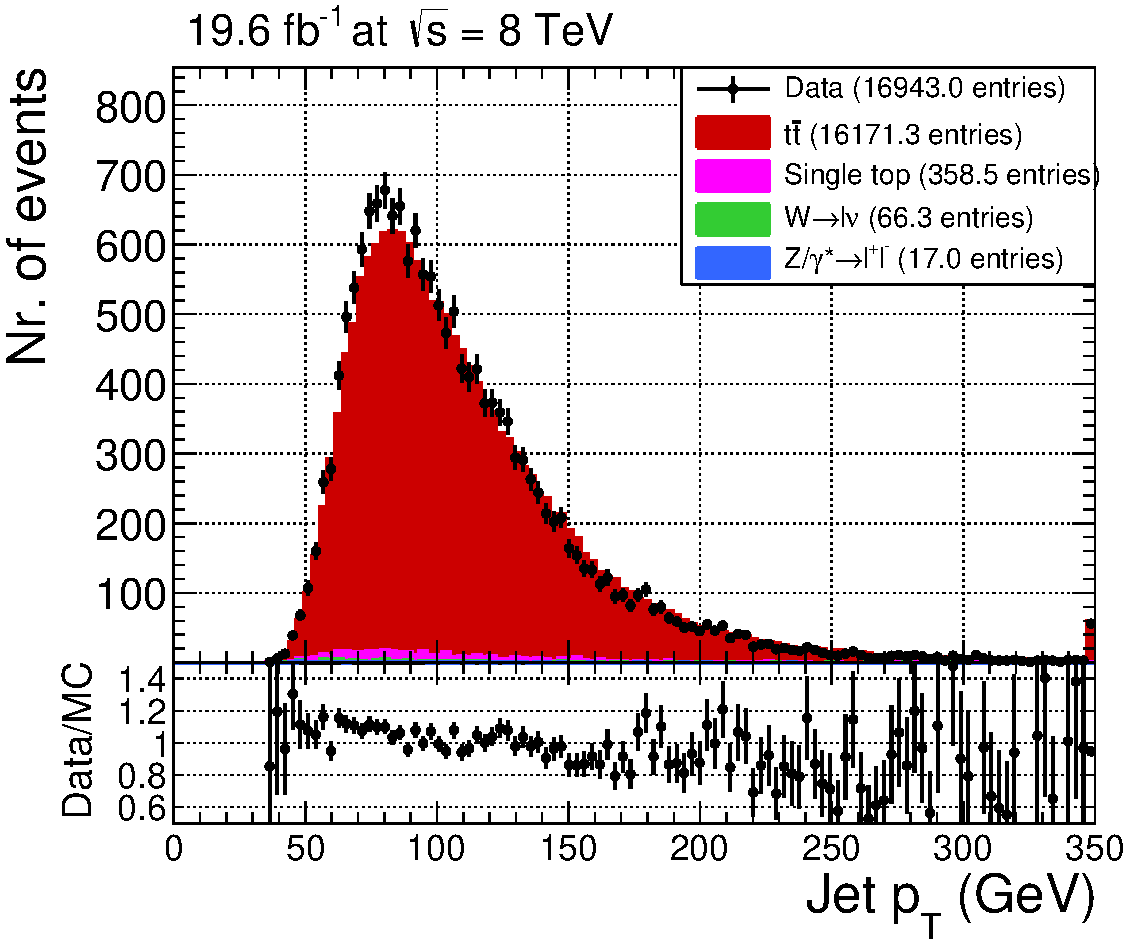
\includegraphics[width = 0.45 \textwidth]{Chapters/Chapter4_EvtSel/Figures/JetPt_LeadingJet_AllCuts_mu_Stack.pdf}
 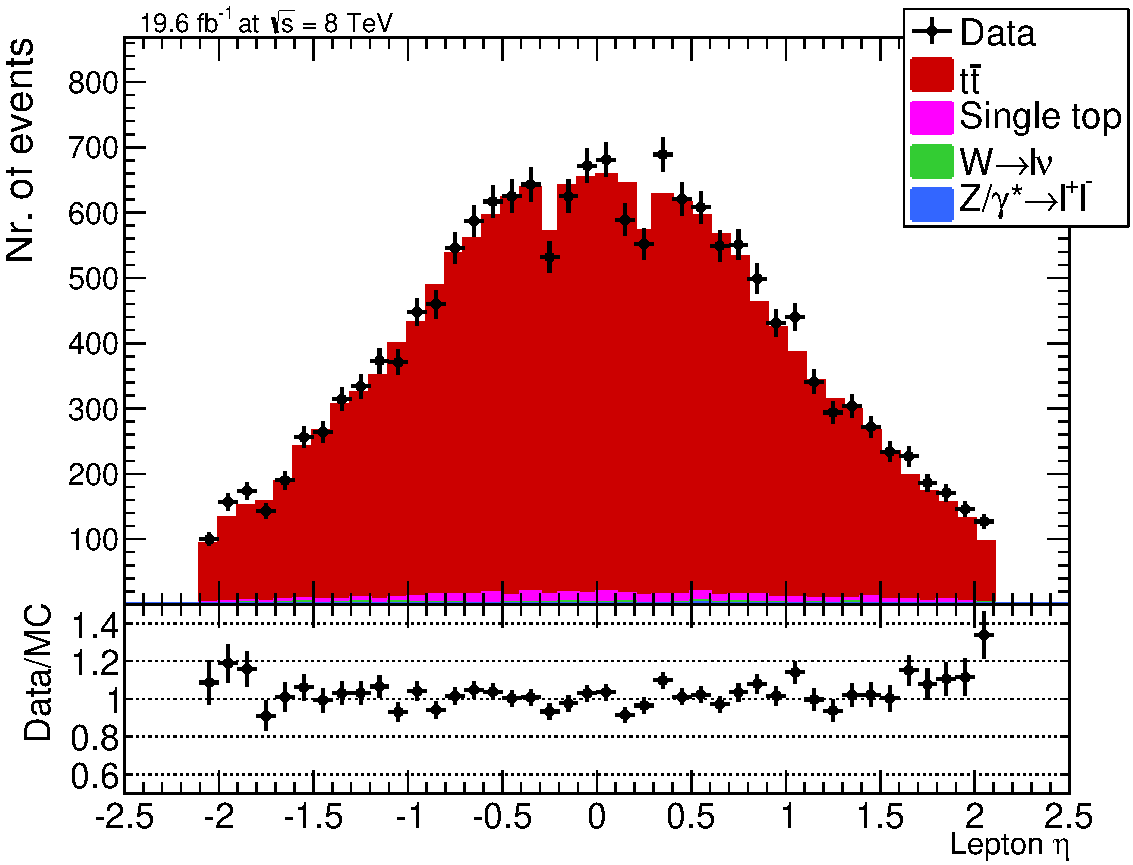
\includegraphics[width = 0.45 \textwidth]{Chapters/Chapter4_EvtSel/Figures/LeptonEta_AllCuts_mu_Stack.pdf}
 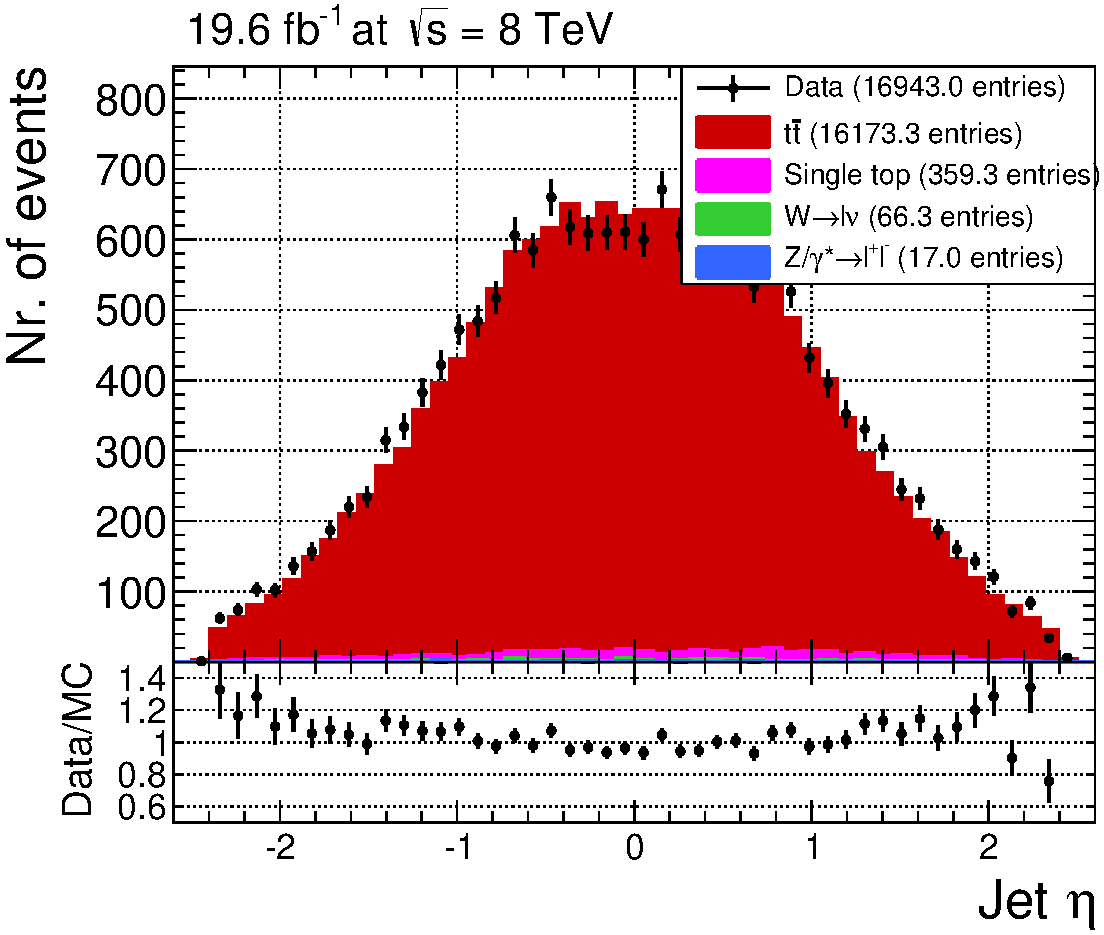
\includegraphics[width = 0.45 \textwidth]{Chapters/Chapter4_EvtSel/Figures/JetEta_LeadingJet_AllCuts_mu_Stack.pdf}
 \caption{Comparison between data and simulation for the lepton transverse momentum (left) and pseudo-rapidity (right) for the two reconstructed light-quark jets. These two jets cannot be differentiated and are therefore permutation left in the considered jet combination.} \label{fig::MSPlots}
\end{figure}

%\begin{table}[h!t]
% \centering
% \caption{b-tag efficiency for the different working points of the CSV b-tagger.}
% \begin{tabular}{c|c|c|c|c}
%  b-tag working point 	& b-jet efficiency 	& udscg efficiency 	& c-jet efficiency 	& udsg efficiency 	\\
%  \hline
%  double Loose 	& 83.79 $\%$		& 18.91 $\%$		& 42.44 $\%$ 		& 13.4 $\%$		\\
%  double Medium 	& 68.71 $\%$		& 4.57 $\%$		& 18.88 $\%$		& 1.21 $\%$		\\
%  double Tight 	& 52.11 $\%$ 		& 1.22 $\%$ 		& 5.74 $\%$ 		& 0.16 $\%$ 		\\
% \end{tabular}
%\end{table}

%\begin{table}[h!t]
% \centering
% \begin{tabular}{c|c|c|c}
%		& $\hat{M_{lb}}$ ($\GeV$) 	& $\hat{M_{qqb}}$ ($\GeV$) 	& $\hat{M_{W}}$ ($\GeV$) 	\\
%  \hline
%  no b-tag 	& 106.9388 $\pm$ 32.0410 	& 174.5792 $\pm$ 17.5196 	& 83.7810 $\pm$ 10.2311 	\\
%  b-tag 	& 107.7945 $\pm$ 32.4255 	& 175.0311 $\pm$ 17.0589 	& 83.6161 $\pm$ 10.2171 	
% \end{tabular}
% \caption{Obtained masses from Gaussian fit on distribution obtained before and after the application of the b-tagging requirement.}
%\end{table}

%\begin{figure}[h!t]
% \centering
% 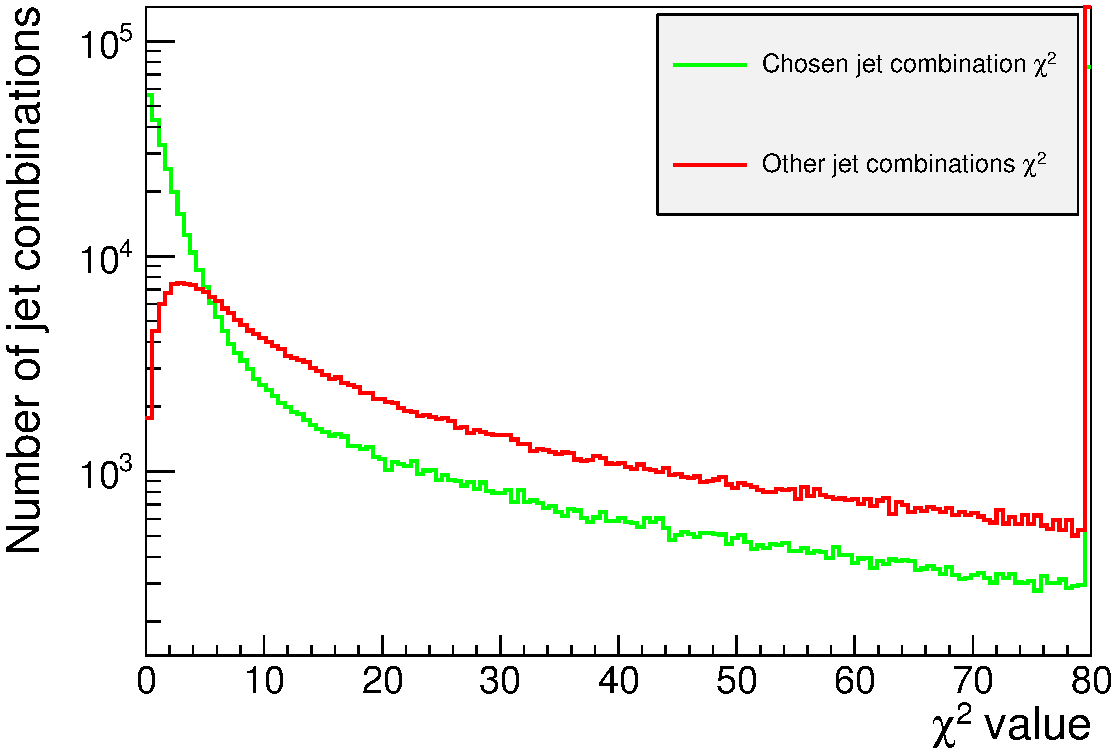
\includegraphics[width = 0.45 \textwidth]{Chapters/Chapter4_EvtSel/Figures/GoodVsBadChiSq_4Jets.pdf}
 %\includegraphics[width = 0.45 \textwidth]{Chapters/Chapter4_EvtSel/Figures/GoodVsBadChiSq.pdf}
 %\caption{Difference between good and wrong jet combinations (also create this for 5-jet case). ... Is this in any way relevant??} \label{fig::GoodVsBadChiSq}
%\end{figure}

%\textit{And will also need to get these numbers for muon channel events alone ... Currently everything is done for muon and electron channel combined!}

